\documentclass[8pt]{beamer}

%%pacotes referentes ao Beamer
%\useoutertheme{split}
%\setbeamertemplate{navigation symbols}{}

%\usetheme{beamertheme}
%\usebeamercolor{beamer-color name}

%\usetheme{Boadilla}
%\usecolortheme{dove}

\usetheme{Montpellier}
\usecolortheme{beaver}

% \usetheme{pittsburgh}
% \usecolortheme{dolphin}
%\usecolortheme{dove}
%\usecolortheme{seahorse}

%\usetheme{Montpellier}

%number in figures an tables -- beamer
\setbeamertemplate{caption}[numbered]

%Colocar no description
%[leftmargin=!,labelwidth=\widthof{Turma A}]
	
%pacotes usuais do latex
\usepackage[portuguese]{babel}
\usepackage[utf8]{inputenc}
\usepackage{bm}
\usepackage{graphicx}
\usepackage{subfig}
\usepackage[round]{natbib}
\usepackage{tikz}
\usetikzlibrary{shapes,arrows}
\usepackage{natbib}
\usepackage{times}
\usepackage{calc} %computes the length of a string
\usepackage{dsfont} %pacote para o 1 estilisado para indicadora
\usepackage{enumerate} %permite fazer uns enumerates diferentes
\usepackage[font=small,labelfont=bf]{caption} %permite colocar um segundo caption
\usepackage{booktabs} % comando \toprule, \midrule e \bottomrule
\usepackage{times} %times new roman font
\usepackage{multirow} %comando \multirow
\usepackage{setspace}
\usepackage{xcolor} %texto colorido
\usepackage{booktabs} %costumized tabs
\usepackage{physics} %absolute value
\usepackage{xcolor}
\usepackage{bigints}
\usepackage{ulem}

% setting color
\definecolor{important}{RGB}{0,153,0}


\usepackage{listings}

\definecolor{codegreen}{rgb}{0,0.6,0}
\definecolor{codegray}{rgb}{0.5,0.5,0.5}
\definecolor{codepurple}{rgb}{0.58,0,0.82}
\definecolor{backcolour}{rgb}{0.95,0.95,0.92}

\lstdefinestyle{mystyle}{
	backgroundcolor=\color{backcolour},   
	commentstyle=\color{codegreen},
	numberstyle=\tiny\color{codegray},
	stringstyle=\color{codepurple},
	basicstyle=\ttfamily\footnotesize,
	breakatwhitespace=false,         
	breaklines=true,                 
	captionpos=b,                    
	keepspaces=true,                 
	numbers=left,                    
	numbersep=5pt,                  
	showspaces=false,                
	showstringspaces=false,
	showtabs=false,                  
	tabsize=2
}

\lstset{style=mystyle}

\renewcommand{\lstlistingname}{Código}% Listing -> Código
\renewcommand{\lstlistlistingname}{Lista de \lstlistingname s}% List of Listings -> List of Código



%código para alinhar a esquerda os itens no description
\defbeamertemplate{description item}{align left}{\insertdescriptionitem\hfill}
\defbeamertemplate{enumerate item}{align left}{\insertdescriptionitem\hfill}

%AMS packages
\usepackage{amsmath}
\usepackage{amsfonts}
\usepackage{amssymb}

%Não quebre linhas
\binoppenalty=\maxdimen
\relpenalty=\maxdimen

%Comandos criados por mim
\DeclareMathOperator*{\argmin}{arg\,min}

\DeclareMathOperator*{\argmax}{arg\,max}


\DeclareMathOperator{\espe}{E}

\DeclareMathOperator{\spann}{span}

\DeclareMathOperator{\cov}{Cov}

\DeclareMathOperator{\vari}{Var}

%Informações para o primeiro slide
\date{}
\title[ANOVA]{Análise de Variância}
\author[Gilberto Sassi]{Gilberto Pereira Sassi}
\institute[IME -- UFBA]{Universidade Federal da Bahia \\ Instituto de Matem\'{a}tica e Estat\'{i}stica\\ Departamento de Estat\'{i}stica }

\begin{document}
	
\tikzstyle{decision} = [diamond, draw, fill=blue!20, 
text width=4.5em, text badly centered, node distance=3cm, inner sep=0pt]
\tikzstyle{block} = [rectangle, draw, fill=blue!20, 
text width=5em, text centered, rounded corners, minimum height=4em]
\tikzstyle{line} = [draw, -latex]
\tikzstyle{cloud} = [draw, ellipse,fill=red!20, node distance=3cm,
minimum height=2em]
	
\begin{frame}{}
	\maketitle
\end{frame}

\section{Comparação de médias: dois tratamentos.}

\begin{frame}{}
Considere $N(\mu_1,\sigma^2)$ e  $N(\mu_2, \sigma^2)$ conforme ilustrado na Figura~\ref{fig:pop-2}.
\begin{figure}[htbp]
	\centering
	\subfloat[][Variáveis aleatórias.]{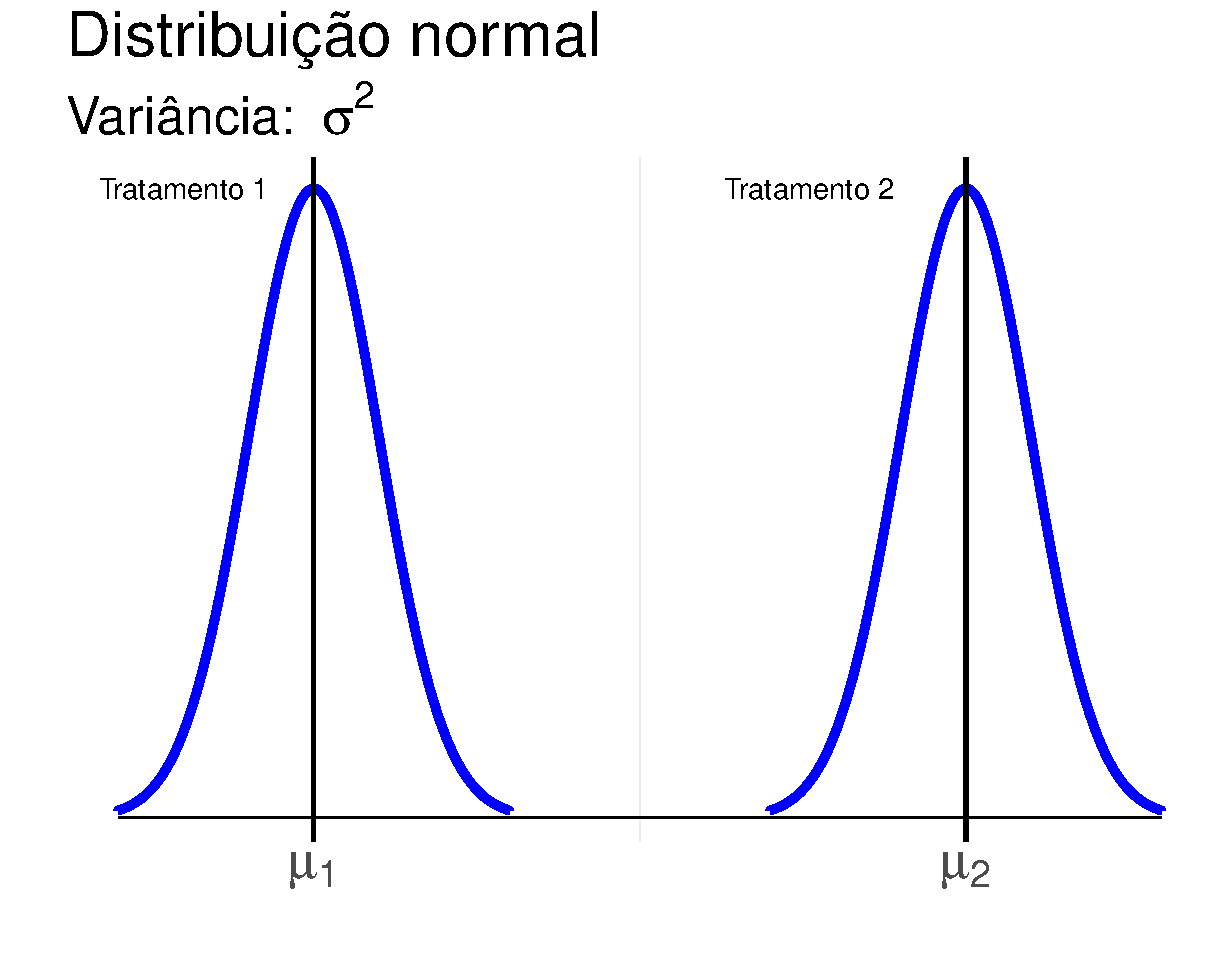
\includegraphics[width=0.4\linewidth]{figure/pop-2.pdf}\label{fig:pop-2}} \hfill
	\subfloat[][Primeira impressão.]{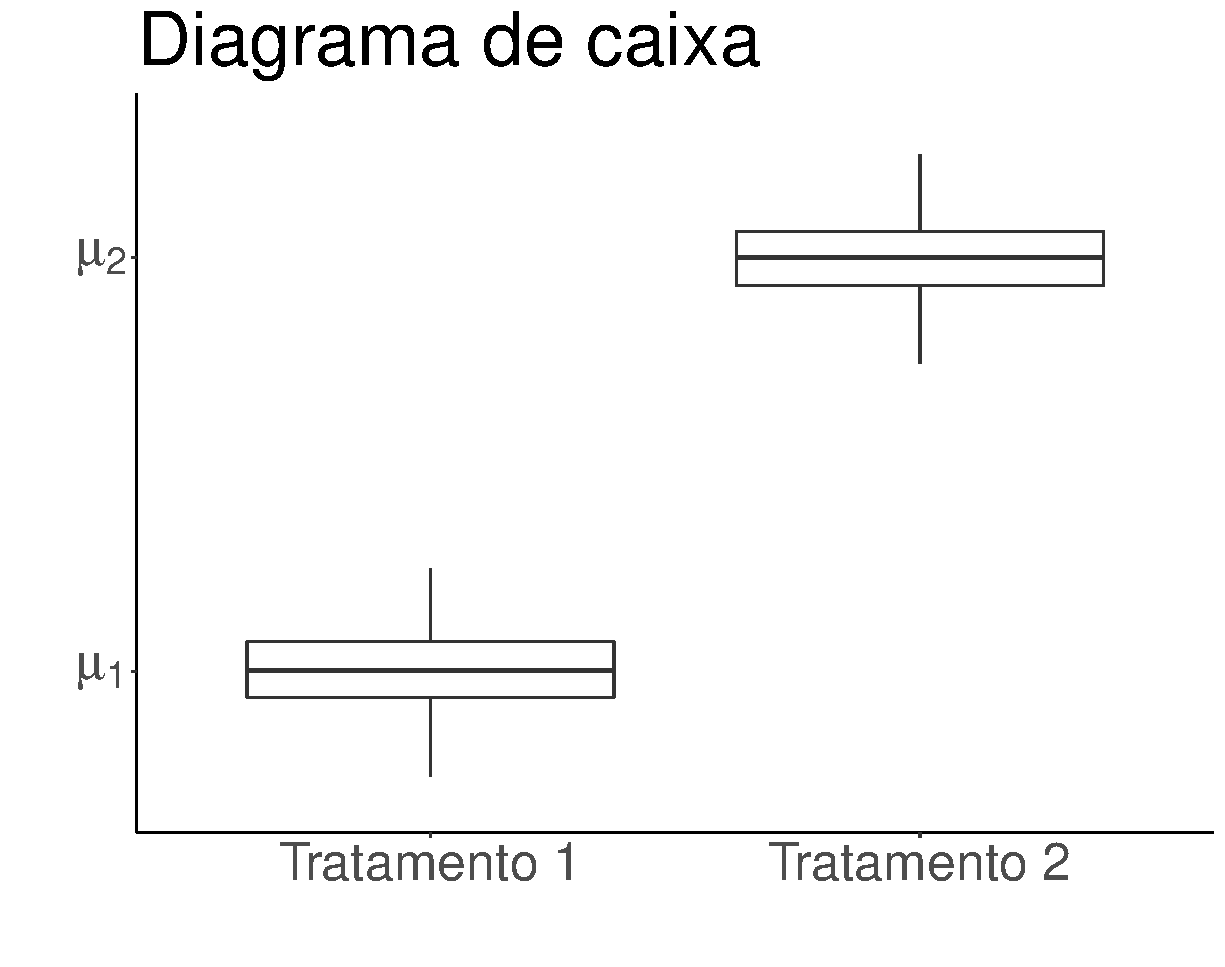
\includegraphics[width=0.4\linewidth]{figure/boxplot-pop-2.pdf}\label{fig:boxplot-pop-2}}
	\caption{Comparação de médias}
\end{figure}

Queremos decidir entre as hipóteses: 
\begin{align*}
H_0: \mu_1 = \mu_2 \qquad \mbox{ e } \qquad H_1: \mu_1 \neq \mu_2,
\end{align*}
Figura~\ref{fig:boxplot-pop-2} nos indica que rejeitaremos $H_0$.

\end{frame}

\section{Comparação de médias: três tratamentos.}

\begin{frame}{}
Considere $N(\mu_1,\sigma^2)$, $N(\mu_2, \sigma^2)$ e  $N(\mu_3, \sigma^2)$ conforme ilustrado na Figura~\ref{fig:pop-3}.
\begin{figure}[htbp]
	\centering
	\subfloat[][Variáveis aleatórias.]{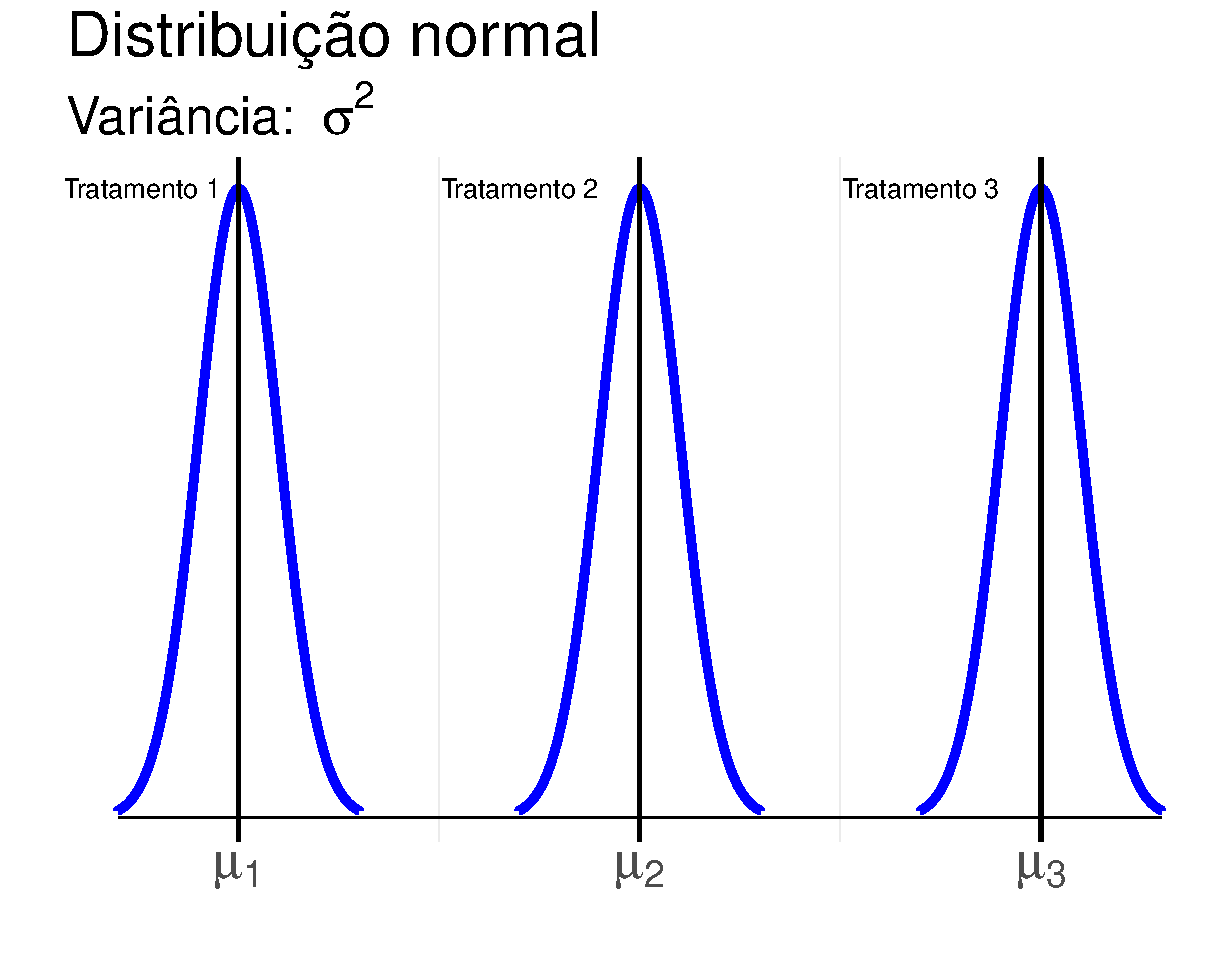
\includegraphics[width=0.4\linewidth]{figure/pop-3.pdf}\label{fig:pop-3}} \hfill
	\subfloat[][Primeira impressão.]{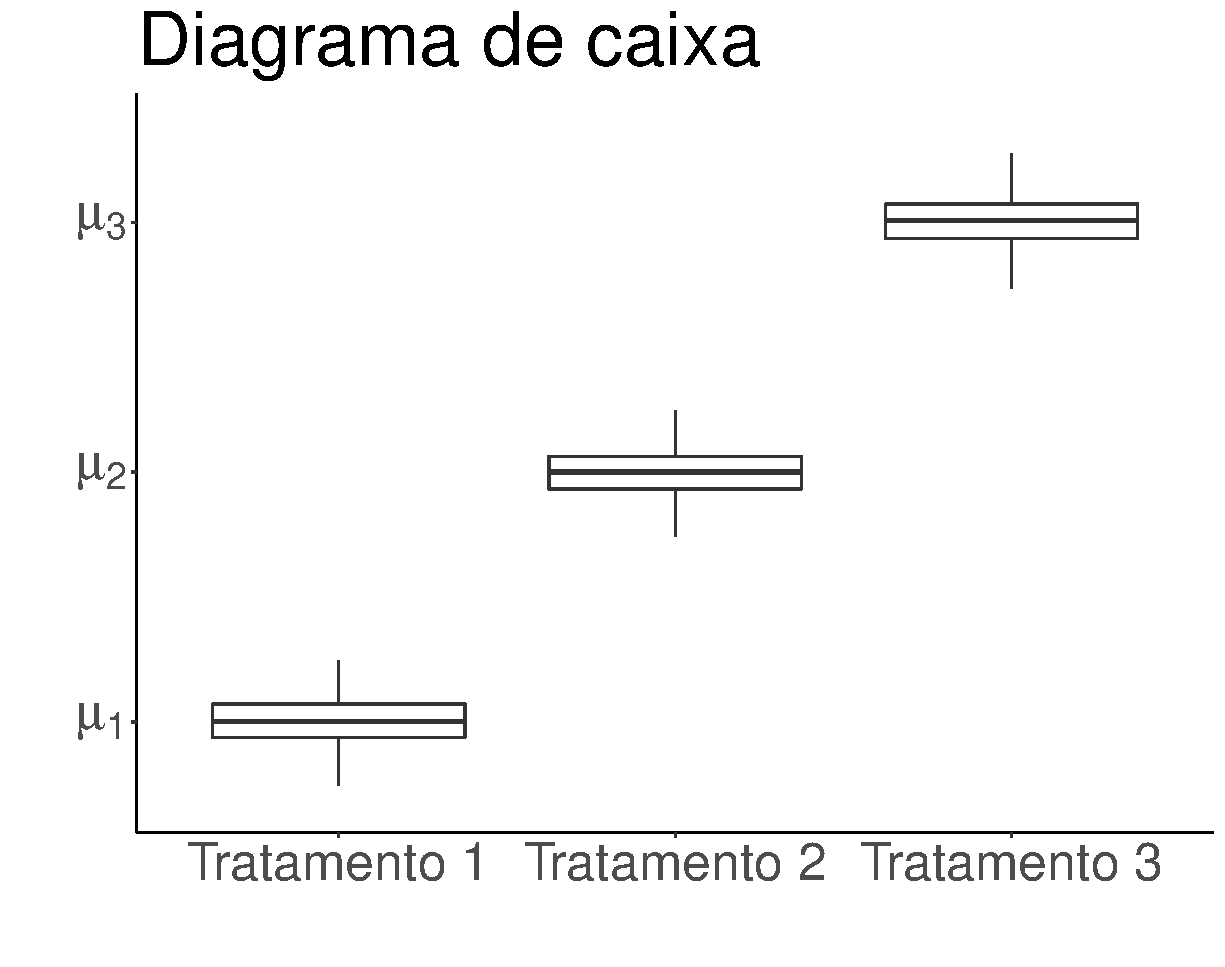
\includegraphics[width=0.4\linewidth]{figure/boxplot-pop-3.pdf}\label{fig:boxplot-pop-3}}
	\caption{Comparação de médias}
\end{figure}

Queremos decidir entre as hipóteses: 
\begin{align*}
H_0: \mu_1 = \mu_2 = \mu_3\mbox{ e }H_1: \mu_i \neq \mu_j, \mbox{ para menos um par }(i, j), i,j\in\{1, 2,3\}, i \neq j,
\end{align*}
Figura~\ref{fig:boxplot-pop-3} nos indica que rejeitaremos $H_0$.

\end{frame}

\section{Estudos completamente aleatórios e balanceados com um fator.}

\begin{frame}{}

\footnotesize
	\begin{itemize}
		\item Suponha que queremos testar $H_0: \mu_1 = \cdots = \mu_a$;
		\item Chamamos $\mu_1, \dots, \mu_a$ de tratamentos;
		\item Imagine que temos uma amostra de tamanho $n$ para cada tratamento: $y_{i1}, \dots, y_{in}, i=1, \dots, a$, conforme ilustrado na Tabela~\ref{fig:dados-anova};
		\begin{table}[htbp]
			\centering
			\scalebox{0.75}{
			\begin{tabular}{c|cccc|c|c}
				\toprule[0.05cm]
				Tratamento & \multicolumn{4}{|c|}{Observações} & Totais & Médias\\ \midrule[0.025cm]
				1 & $y_{11}$ & $y_{12}$ & $\dots$ & $y_{1n}$ & $y_{1\cdot}$ & $\bar{y}_{1\cdot} = \frac{y_{1\cdot}}{n}$\\
				2 & $y_{21}$ & $y_{22}$ & $\dots$ & $y_{2n}$ & $y_{2\cdot}$ & $\bar{y}_{2\cdot} = \frac{y_{2\cdot}}{n}$\\
				$\vdots$ & $\vdots$ & $\vdots$ &  & $\vdots$ & $\vdots$ & $\vdots$\\
				n & $y_{n1}$ & $y_{n2}$ & $\dots$ & $y_{nn}$ & $y_{n\cdot}$ & $\bar{y}_{n\cdot}=\frac{y_{n\cdot}}{n}$\\ \midrule[0.025cm]
				 &  &  &  &  & $y_{\cdot\cdot}$ & $\bar{y}_{\cdot\cdot} = \frac{y_{\cdot\cdot}}{n \cdot a}$\\
				 \bottomrule[0.05cm]
			\end{tabular}
			}
			\caption{Dados de um estudo completamento aleatórios e balanceados com um fator.}
			\label{fig:dados-anova}
		\end{table}
	
		\item  Descrevemos os dados da Tabela~\ref{fig:dados-anova} através de
		\begin{align} \label{eq:anova}
			y_{ij} = \mu + \tau_i + \epsilon_{ij}, \quad \epsilon_{ij} \sim N(0, \sigma^2);
		\end{align}

		\item Queremos testar as seguintes hipóteses
		\begin{align*} 
	 		&H_0: \tau_1 = \tau_2 = \dots = \tau_a = 0,\\
			&H_1: \tau_i \neq 0 \mbox{ para pelo menos um }i, i\in \{1, 2, \dots, a\}. 
		\end{align*}
	\end{itemize}
	Chamamos $\tau_i, i=1, \dots, a$ de efeitos do tratamentos.
\end{frame}

\begin{frame}{Soma dos quadrados.}

Note que
\normalsize 
\begin{align*}
SS_{T} &= \underbrace{\sum_{i=1}^{a} \sum_{j=1}^{n} (y_{ij} - \bar{y}_{\cdot \cdot})^2}_{\mbox{Soma dos quadrados total}} = (N-1)s^2\\
&= \underbrace{ \sum_{i=1}^{a} n (\bar{y}_{i\cdot} - \bar{y}_{\cdot \cdot})^2 }_{\mbox{Soma dos Quadrados dos Tratamentos}} + \underbrace{\sum_{i=1}^{a} \sum_{j=1}^{n} (y_{ij} - \bar{y}_{i\cdot})^2 }_{\mbox{Soma dos Quadrados do Erro}}\\
&= \underbrace{\sum_{i=1}^{a} n (\bar{y}_{i \cdot } - \bar{y}_{\cdot \cdot})^2 }_{SQ_{Tratamentos}} + \underbrace{\sum_{i=1}^{a} (n-1) s_i^2}_{SQ_E} = SQ_{Tratamentos} + SQ_E.
\end{align*}
\normalsize
em que
\begin{itemize}
	\item  $s^2 = \frac{1}{N-1} \sum_{i=1}^{a} \sum_{j=1}^{n} (y_{ij} - \bar{y}_{\cdot \cdot})^2$, em que $N = n\cdot a$ (variância total);
	\item $s^2_i = \frac{1}{n-1} \sum_{j=1}^{n} (y_{ij} - \bar{y}_{i\cdot})^2$ (variância do tratamento $i$).
\end{itemize}
Se $H_0: \tau_1 = \tau_2 = \dots = \tau_a = 0$ é verdadeira, então $Y_{ij} \sim N(\mu, \sigma^2), \forall i,j$.
\end{frame}

\begin{frame}{Quadrado médio.}

Usando a equação~\eqref{eq:anova}, podemos provar que 
\begin{itemize}
	\item $\espe\left(SQ_{Tratamentos}\right) = (a-1) \sigma^2 +  n \cdot \tau_1^2 + \cdots + n \cdot \tau_a^2$;
	\item $\espe\left( SQ_E \right) = (N - a ) \sigma^2$;
	\item Quadrado Médio dos Tratamentos: $QM_{Tratamentos} = \frac{SQ_{Tratamentos}}{a-1}$;
	\item Quadrado Médio do Erro: $QM_E = \frac{SQ_{E}}{N-a}$;
	\item $F_0 = \frac{QM_{Tratamentos}}{QM_E}$.
\end{itemize}
\vfill

É possível provar que 
\begin{itemize}
	\item $\espe\left(QM_{Tratamentos}\right) = \sigma^2 + \frac{n \cdot \tau_1^2 + \cdots + n \cdot \tau_a^2}{a-1}$;
	\item $\espe \left( QM_{E} \right)= \sigma^2$;
\end{itemize}

Rejeitamos $H_0: \tau_1 = \tau_2 = \dots = \tau_a = 0$ se $F_0 = \frac{QM_{Tratamentos}}{QM_E}$ for grande.

Se $H_0$ for verdadeiro, temos que $F_0 \sim F_{a-1, N-a}$, em que $F_{a-1, N-a}$ é a distribuição $F$.

Teste ANOVA é robusto para tratamentos com variâncias ligeiramente diferentes.

\end{frame}

\begin{frame}{ANOVA}
\begin{figure}[htbp]
	\centering
	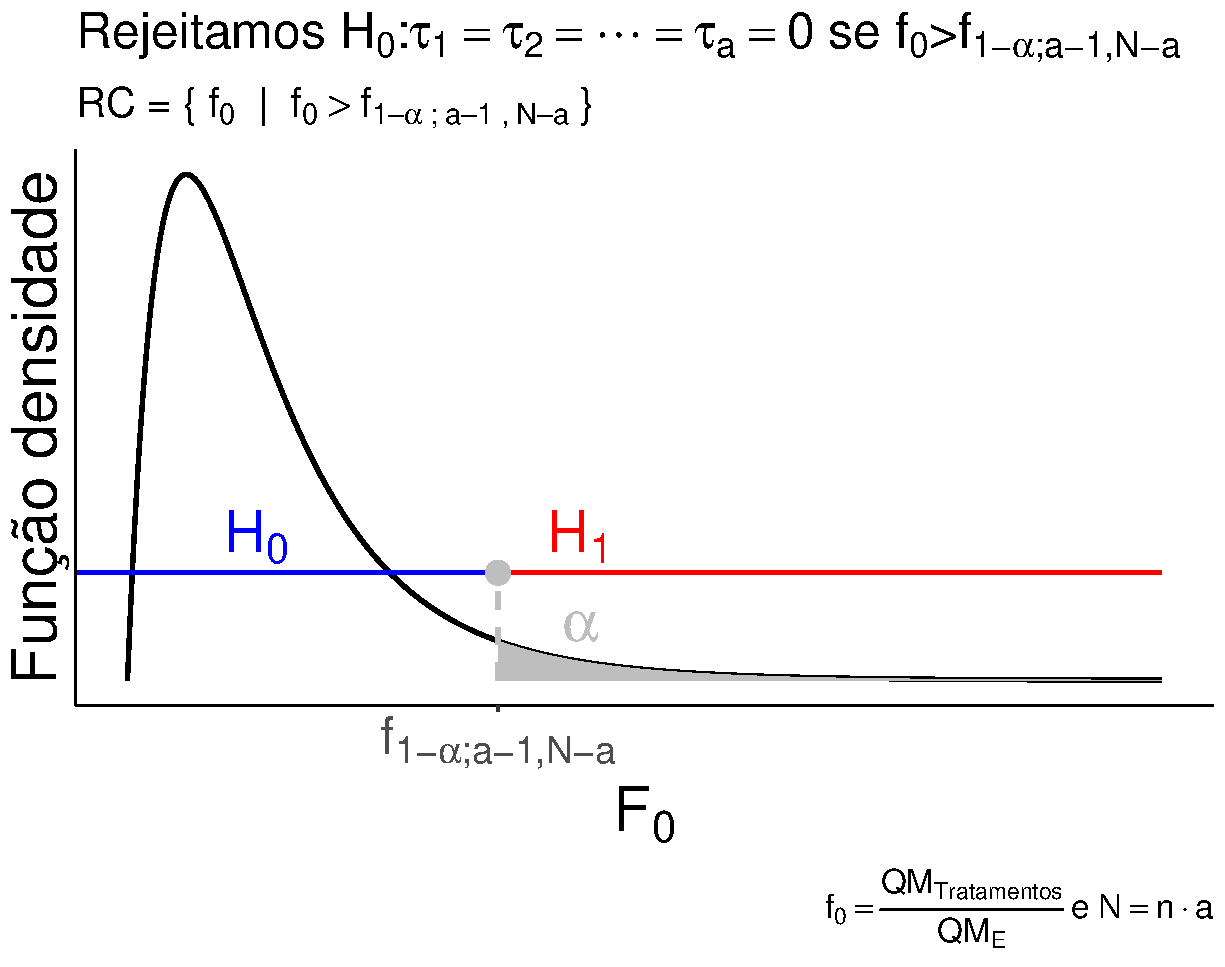
\includegraphics[width=0.70\linewidth]{figure/anova-test.pdf}
	\caption{Região crítica para ANOVA.}
\end{figure}
\end{frame}

\begin{frame}{ANOVA: Checando as suposições do modelo.}

\small
\begin{block}{Análise de resíduo}
	Depois decidir entre $H_0$ e $H_1$, precisamos checar as suposições do modelo:
	\begin{enumerate}[(a)]
		\item $\epsilon_{ij}, j=1, \dots, n, i=1, \dots, a$ são independentes;
		\item $\epsilon_{ij}, j=1, \dots, n, i=1, \dots, a$ tem distribuição normal;
		\item  $\epsilon_{ij}, j=1, \dots, n, i=1, \dots, a$ tem variância constante.
	\end{enumerate} 
	
	$\epsilon_{ij} = y_{ij} - \mu + \tau_i  = y_{ij} - \mu_i, j=1, \dots, n, i=1, \dots, a$ não são observáveis pois não conhecemos as médias populacionais dentro de cada tratamento, mas podemos aproximar estas médias populacionais $\mu_i$ por  $\bar{y}_{i\cdot}, i=1, \dots, a$. Assim, podemos definimos os resíduos por
	\begin{align}\label{eq:residuo-balanced}
	e_{ij} = y_{ij} - \bar{y}_{i\cdot}, j=1, \dots, n, i=1, \dots, a.
	\end{align}
	
	Usando a equação~\eqref{eq:residuo-balanced}, podemos usar gráficos para checar \textcolor{blue}{(a)}, \textcolor{blue}{(b)} e \textcolor{blue}{(c)}:
	\begin{enumerate}[(a)]
		\item \textbf{Independência:} cada par $(i+j, e_{ij}), j=1, \dots, n, i=1, \dots, a,$ é representado por um ponto no plano cartesiano. Se não existe padrão ou tendência,então assumimos que $\epsilon_{ij}$ são independentes;
		\item \textbf{Normalidade:} cada par $\left( q_{(i+j)}; \frac{e_{(i+j)} - \bar{e}_{\cdot\cdot}}{s_e}  \right)$$, j=1, \dots, n, i=1, \dots, a$ é representado por um ponto no plano cartesiano, em que $\Phi(q_{(i+j)}) = \frac{i+j-0,5}{n}$ e $s_e$ é o desvio padrão dos resíduos -- este gráfico é chamado de gráfico de probabilidade normal. Se os pontos estão próximos ou em cima da reta $y=x$, então $\epsilon_{ij}$ tem distribuição normal;
		\item \textbf{Variância constante:} cada par $\left(  \bar{y}_{i\cdot}, e_{ij} \right), j=1, \dots, n, i=1, \dots, a,$ é representando por um ponto no plano cartesiano. Se não existe padrão ou tendência, então assumimos que $\epsilon_{ij}$ tem variância constante.
	\end{enumerate}
\end{block}
\normalsize

\end{frame}


\begin{frame}{ANOVA}

\begin{block}{Exemplo}
	Em um experimento que deseja analisar se a resistência à tração de um tecido está associada com a porcentagem da fibra de algodão. Cinco níveis de porcentagem da fibra de algodão e cinco observações em cada nível de porcentagem de fibra de algodão. Os dados estão na Tabela~\ref{tab:resistencia}. Desenhe diagramas de caixa para cada nível de porcentagem de algodão. A porcentagem de algodão afeta a resistência à tração do tecido? Use $\alpha = 5\%$. Calcule o valor-p.
	\begin{table}[ht]
		\centering
		\scalebox{0.65}{
		\begin{tabular}{c|ccccc|c|c}
			\toprule[0.05cm]
			Algodão & \multicolumn{5}{|c|}{Observações} & Total & Variância em cada tratamento \\ 
			\midrule[0.025cm]
			15 &   7 &   7 &  15 &  11 &   9 &  49 & 11,20 \\ 
			20 &  12 &  17 &  12 &  18 &  18 &  77 & 9,80 \\ 
			25 &  14 &  18 &  18 &  19 &  19 &  88 & 4,30 \\ 
			30 &  19 &  25 &  22 &  19 &  23 & 108 & 6,80 \\ 
			35 &   7 &  10 &  11 &  15 &  11 &  54 & 8,20 \\ \midrule[0.025cm]
			\multicolumn{7}{r|}{}   & Variância total = 26,54\\
			\bottomrule[0.05cm]
		\end{tabular}
		}
		\caption{Resistência à tração} 
		\label{tab:resistencia}
	\end{table}
\end{block}

\end{frame}

\begin{frame}{ANOVA}

\begin{block}{Solução}
	\begin{figure}[htbp]
		\centering
		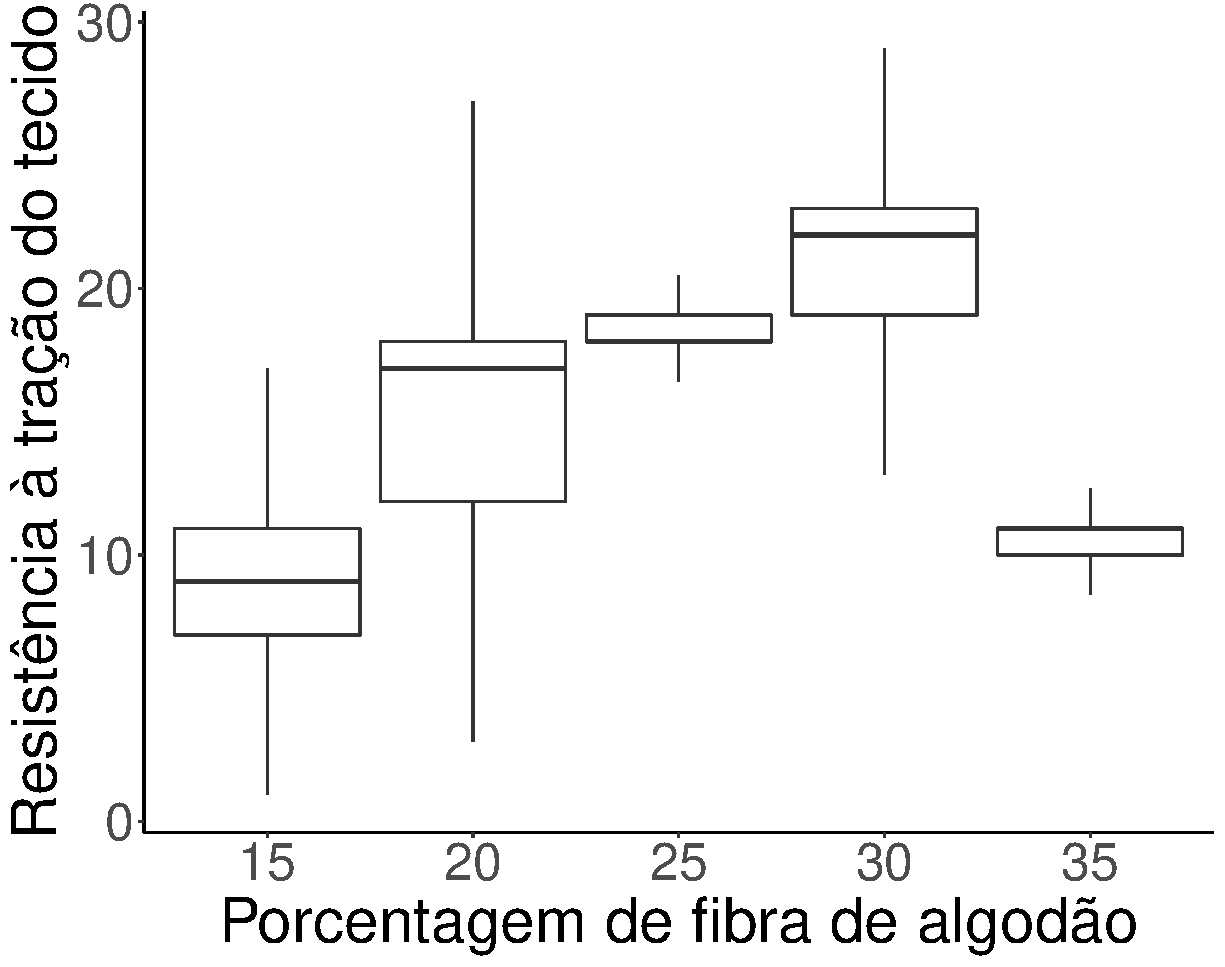
\includegraphics[width=0.65\linewidth]{figure/boxplot-ex1.pdf}
		\caption{Diagrama de caixa com nível de porcentagem de algodão.}
	\end{figure}
\end{block}

\end{frame}

\begin{frame}{ANOVA}

\footnotesize
\begin{block}{Solução}
	As médias populacionais de resistência à tração com porcentagem de fibra algodão são: $\mu_{15} = \mu + \tau_{15}$, $\mu_{20} = \mu + \tau_{20}$, $\mu_{25} = \mu + \tau_{25}$, $\mu_{30} = \mu + \tau_{30}$ e $\mu_{35} = \mu + \tau_{35}$.
	
	\textbf{Passo 1)} Queremos testar as hipóteses: $H_0: \tau_{15} = \tau_{20} = \tau_{25} = \tau_{30} = \tau_{35} = 0$ e $H_1: \tau_{15}^2 + \tau_{20}^2 + \tau_{25}^2 + \tau_{30}^2 + \tau_{35}^2 > 0$;
	
	\textbf{Passo 2)} Nível de significância $\alpha=5\%$;
	
	\textbf{Passo 3)} Rejeitamos $H_0$ se $F_0 = \frac{QM_{Tratamentos}}{QM_E}$ for grande. Ou seja, $RC = \left\{ f_0 \mid f_0 > f_{1-\alpha; a-1, N-a} \right\}$, em que $N=a \cdot n = 5 \cdot 5 = 25$ e $a = 5$;
	
	\textbf{Passo 4)} Vamos encontrar o valor crítico:
	\begin{itemize}
		\item $P(F_{a-1, N-a} \leq f_{1-\alpha; a-1, N-a}) = P(F_{4, 20} \leq f_{0,95; 4, 20}) = 1-\alpha=0,95$, então $f_{0,95; 4, 20} = 2,8661$;
	\end{itemize}

	\textbf{Passo 5)} Na Tabela~\ref{tab:anova-table-ex1}, mostramos a soma dos quadrados e os quadrados médios:
	\begin{table}[ht]
		\centering
		\scalebox{0.65}{
		\begin{tabular}{l|l|l|l|l}
			\toprule[0.05cm]
			Fonte de variação & Graus de liberdade & Soma dos Quadrados & Quadrados Médios & $F_0$  \\ 
			\midrule[0.025cm]
			Tratamentos     & $a-1= 4$ & $SQ_{Tratamentos} = 475,76$ & $QM_{Tratamentos} =  118,94$ & $\frac{QM_{Tratamentos}}{QM_E} = 14,76$  \\ 
			Erro   & $N-a= 20$ & $SQ_E = 161,20 =  (n-1)s_1^2+(n-1)s_2^2+(n-1)s_3^2+(n-1)s_4^2 $ & $QM_E=8,06$   &  \\ \midrule[0.025cm]
			Total & $N-1=24$ & $SQ_T = 636,96 = (N-1)s^2$ & & \\
			\bottomrule[0.05cm]
		\end{tabular}
		}
		\caption{\scriptsize Tabela ANOVA.} 
		\label{tab:anova-table-ex1}
	\end{table}
	Como $F_0 = 14,76 > f_{0,95; 4, 20} = 2,8661$, rejeitamos $H_0$, ou seja, ao nível de significância $\alpha=5\%$ as resistências médias não são iguais para os diferentes níveis de porcentagem de fibra de algodão.
	
\end{block}
\normalsize

\end{frame}

\begin{frame}{ANOVA}

\begin{block}{Solução (valor-p)}
	O valor-p é dado por
	$$p=P(F_0 > f_0 \mid H_0) = 1 - P(F_{a-1, N-a} < f_0).$$
	
	Usando as informações da Tabela~\ref{tab:anova-table-ex1}, temos que $f_0 = 14,76$. Então, o valor-p é dado por
	\begin{align*}
		p &= 1 - P(F_{a-1, N-a} \leq f_0)\\
		&= 1 - P(F_{4, 20} \leq 14,76)\qquad \textcolor{important}{\mbox{Calculei usando o R}}\\
		&= 1 - 1\\
		&=0
	\end{align*}
	
	Como $p=0 < \alpha = 0,05$, rejeitamos $H_0$. Então, as resistências médias não são iguais para os diferentes níveis (15, 20, 25, 30 e 35) de porcentagem de fibra de algodão.
\end{block}
\end{frame}

\begin{frame}{ANOVA}

\begin{block}{Solução (Análise de resíduos)}
	Primeiro calculamos os resíduos e médias dentro de cada tratamento:
		\begin{table}[ht]
		\centering
		\scalebox{0.8}{
			\begin{tabular}{c|ccccc|c|c}
				\toprule[0.05cm]
				Algodão & \multicolumn{5}{|c|}{Resíduos} & Média em cada tratamento & Variância em cada tratamento \\ 
				\midrule[0.025cm]
				15 &   -2,8 & -2,8 & 5,2 & 1,2 & -0,8 &  9,80 & 11,20 \\ 
				20 &  -3,4 & 1,6 & -3,4 & 2,6 & 2,6 &  15,40 & 9,80 \\ 
				25 &  -3,6 & 0,4 & 0,4 & 1,4 & 1,4 &  17,60 & 4,30 \\ 
				30 &  -2,6 & 3,4 & 0,4 & -2,6 & 1,4 & 21,60 & 6,80 \\ 
				35 &   -3,8 & -0,8 & 0,2 & 4,2 & 0,2 &  10,80 & 8,20 \\ \midrule[0.025cm]
				\multicolumn{7}{r|}{}   & Variância total = 26,54\\
				\bottomrule[0.05cm]
			\end{tabular}
		}
		\caption{Resistência à tração} 
		\label{tab:resistencia-residuos}
	\end{table}

	\begin{enumerate}[(a)]
		\item Na Figura~\ref{fig:qqnorm-balanced-ex1}, os pontos estão próximos perto da reta $y = x$ e concluímos que $\epsilon_{ij}$ tem distribuição normal;
		\item Na Figura~\ref{fig:independence-balanced-ex1}, não existe padrão ou tendência e concluímos que $\epsilon_{ij}$ são independentes;
		\item Na Figura~\ref{fig:variance-balanced-ex1}, não existe padrão ou tendência e concluímos que  $\epsilon_{ij}$ tem variância constante.
	\end{enumerate}
\end{block}
\end{frame}

\begin{frame}{ANOVA}

\begin{block}{Análise de resíduo}
	\begin{figure}[htbp]
		\centering
		\subfloat[Gráfico de probabilidade normal.]{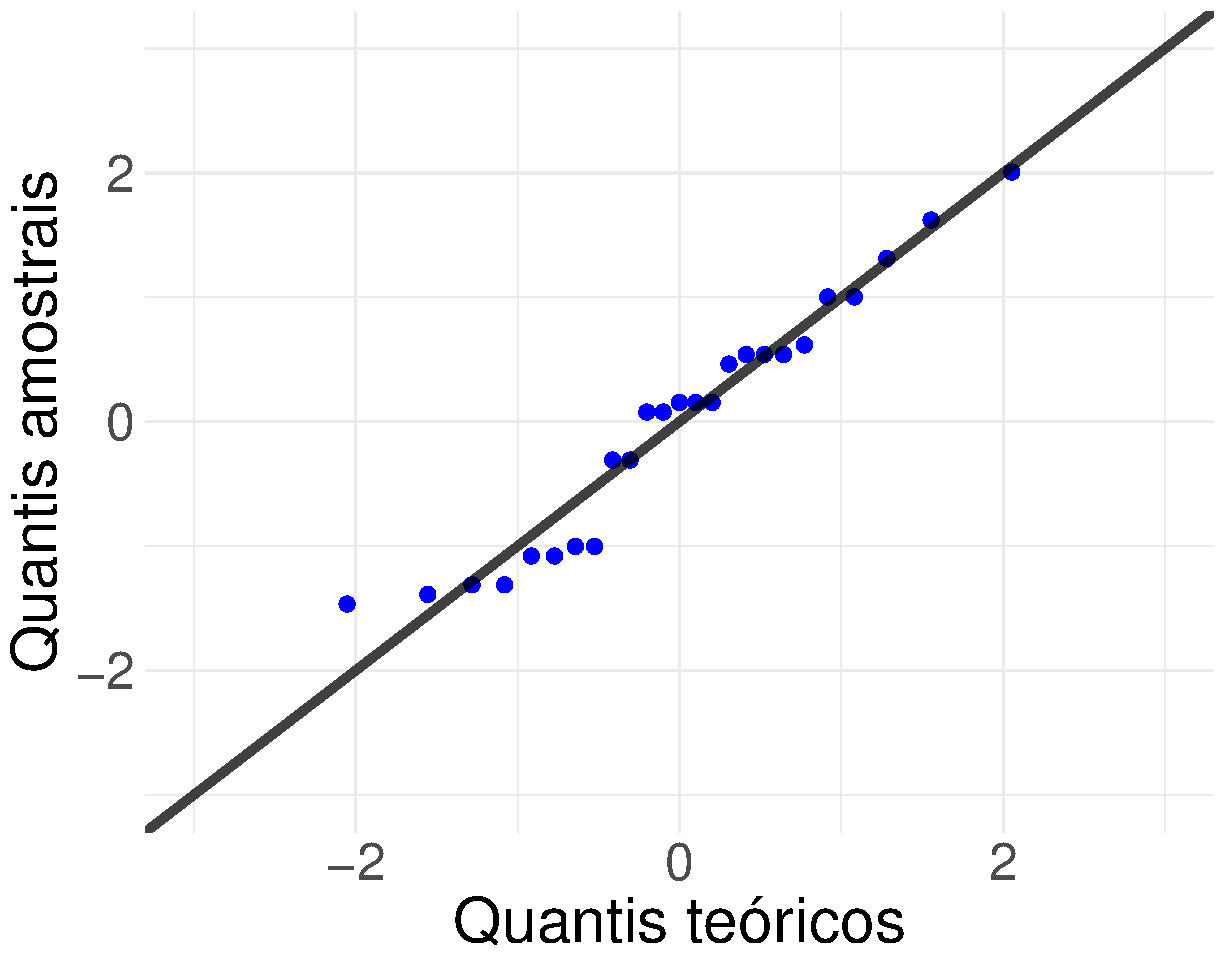
\includegraphics[width=0.33\linewidth]{figure/qqnorm-balanced-ex1.pdf} \label{fig:qqnorm-balanced-ex1}}
		\subfloat[Tempo $\times$ Resíduos.]{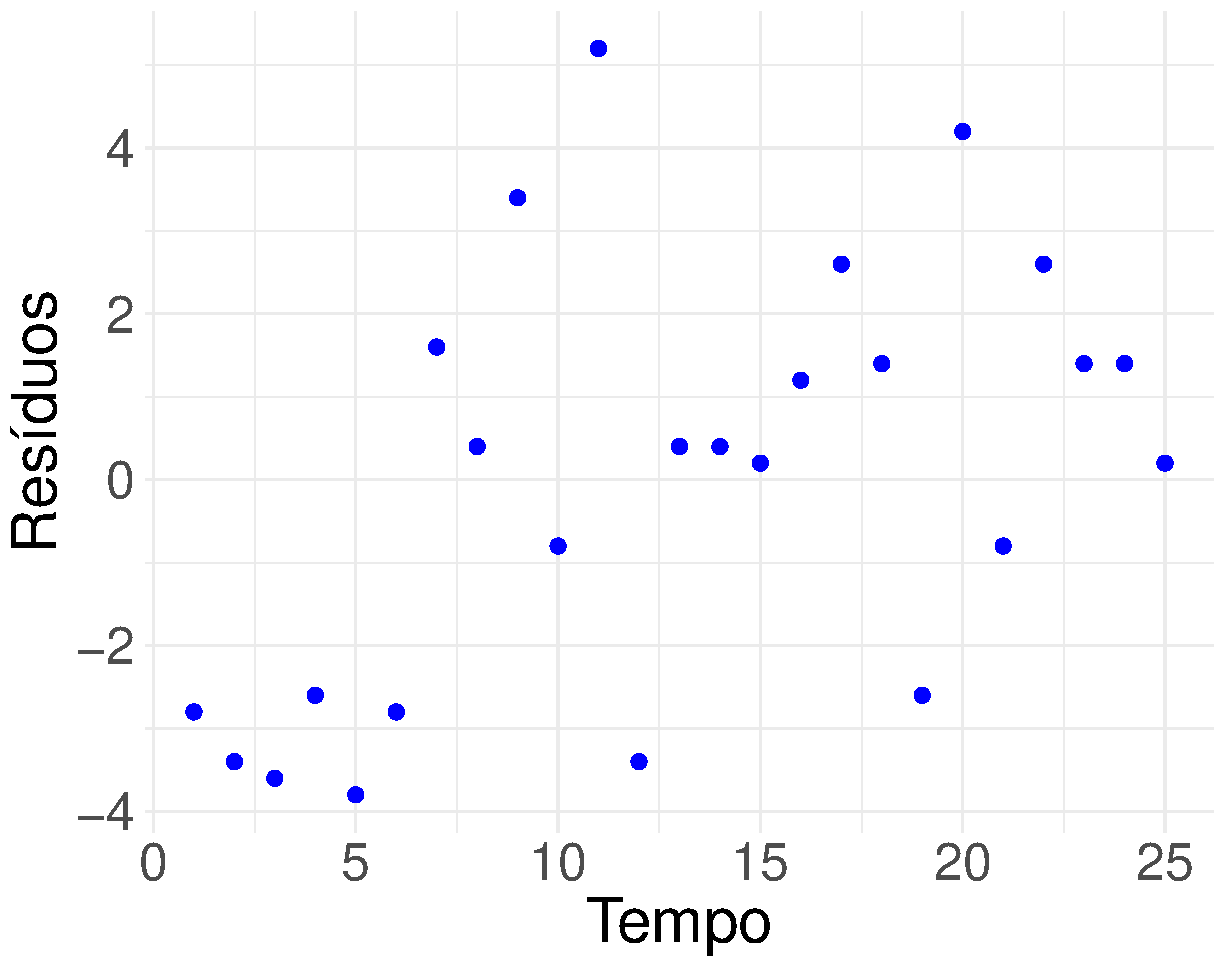
\includegraphics[width=0.33\linewidth]{figure/independence-balanced-ex1.pdf} \label{fig:independence-balanced-ex1}}
		\subfloat[$\bar{y}_{i\cdot}$ $\times$ Resíduos.]{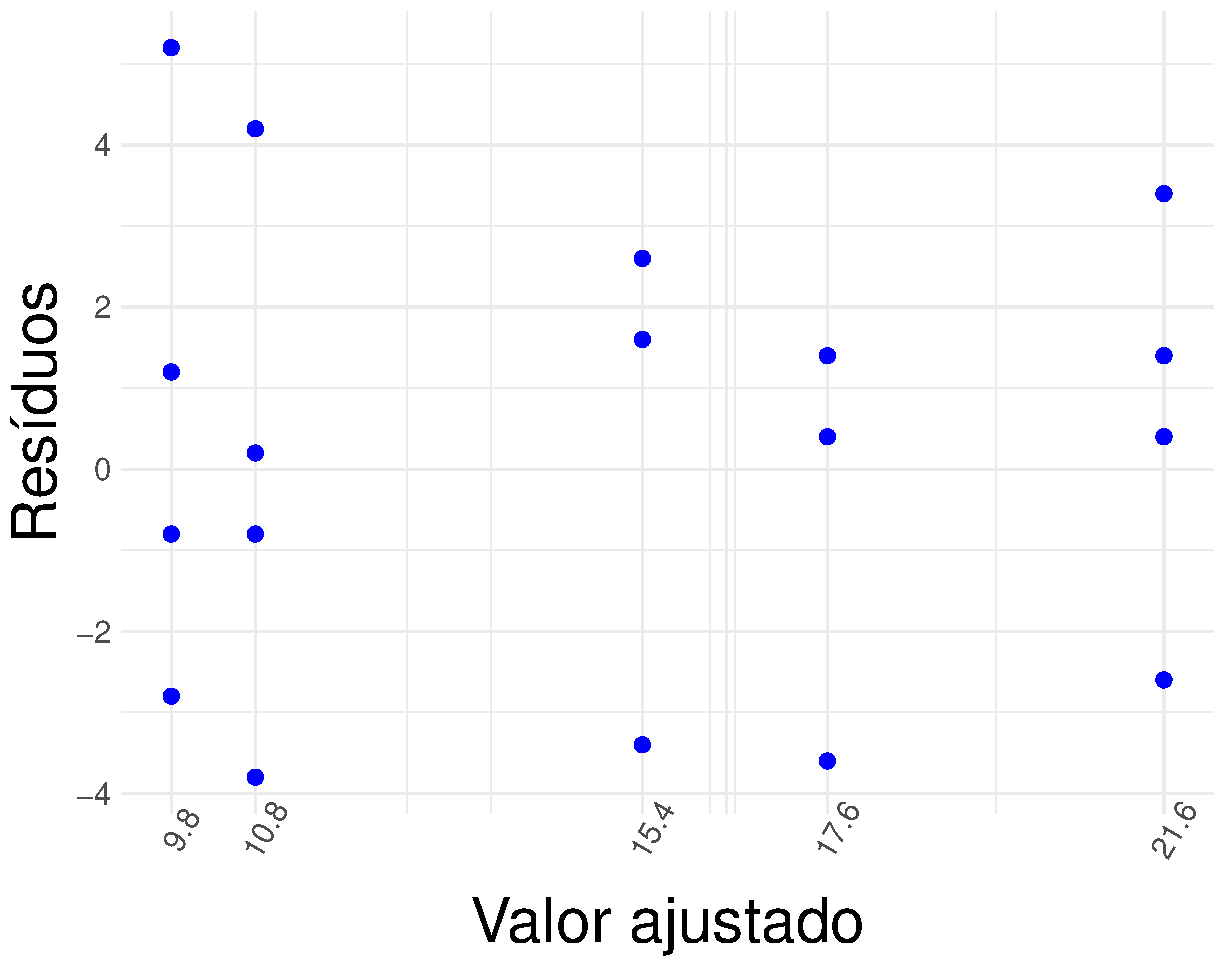
\includegraphics[width=0.33\linewidth]{figure/variance-balanced-ex1.pdf} \label{fig:variance-balanced-ex1}}
		\caption{Análise de resíduos.}
	\end{figure}
\end{block}

\end{frame}	


\begin{frame}{ANOVA}
\begin{block}{Exemplo}
	Imagine que um pesquisador realizou um experimento completamente aleatório e balanceado para checar $a$ tratamentos ou níveis de um fator. Algumas informações do experimento estão na Tabela~\ref{tab:anova_table-ex2}. Complete a Tabela~\ref{tab:anova_table-ex2}. As médias dos tratamentos são diferentes? Use $\alpha=5\%$. Calcule o valor-p.
	\begin{table}[htbp]
		\centering
		\scalebox{0.575}{
		\begin{tabular}{l|l|l|l|l}
			\toprule[0.05cm]
			Fonte de variação  & Graus de liberdade & Soma dos Quadrados & Quadrados Médios & $F_0$\\ \midrule[0.025cm]
			Tratamentos & $a-1=3$ & $SQ_{Tratamentos}=?$ & $QM_{Tratamentos} = ?$ & $\frac{QM_{Tratamentos}}{QM_E} = ? $\\ 
			Erro & $N-a = ?$ & $SQ_E =  (n-1)s_1^2 + (n-1)s_2^2 + (n-1)s_3^2 + (n-1)s_4^2 =  396,8$ & $QM_E = ? $ & \\ \midrule[0.025cm]
			Total & $N-1=19$ & $SQ_T = (N-1)s^2 = 514,2$  & \\ \bottomrule[0.05cm]
		\end{tabular}
		}
		\caption{Algumas informações do experimento.}
		\label{tab:anova_table-ex2}
	\end{table}
\end{block}
\end{frame}

\begin{frame}{ANOVA}

\normalsize
\begin{block}{Solução}
	\textbf{Passo 1)} Note que $a = 4$ e queremos testar as seguintes hipóteses: $H_0: \tau_1 = \tau_2 = \tau_3 = \tau_4 = 0$ e $H_1: \tau_1^2 + \tau_2^2 + \tau_3^2 + \tau_4^2 > 0$;
	
	\textbf{Passo 2)} Nível de significância $\alpha=5\%$;
	
	\textbf{Passo 3)} Rejeitamos $H_0$ se $F_0 = \frac{QM_{Tratamentos}}{QM_E}$ for grande. Ou seja, $RC = \left\{ f_0 \mid f_0 > f_{1-\alpha;a-1,N-a} \right\}$.
	
	\textbf{Passo 4)} Note que $N-a = (N-1)  - (a-1) = 16$. Vamos encontrar o valor crítico:
	\begin{itemize}
		\item $P(F_{a-1, N-a} \leq f_{1-\alpha; a-1, N-a}) = P(F_{3, 16} \leq f_{0,95; 3, 16}) = 1- \alpha = 0,95$, então $f_{0,95; 3, 16} = 3,2389$.
	\end{itemize}

	\textbf{Passo 5)} Completamos as informações da Tabela~\ref{tab:anova_table-ex2} na Tabela~\ref{tab:anova_table-ex2-comp}.
	\begin{table}[htbp]
		\centering
		\scalebox{0.5}{
			\begin{tabular}{l|l|l|l|l}
				\toprule[0.05cm]
				& Graus de liberdade & Soma dos Quadrados & Quadrados Médios & $F_0$\\ \midrule[0.025cm]
				Tratamentos & $a-1=3$ & $SQ_{Tratamentos}=514,2 - 396,8=117,4$ & $QM_{Tratamentos} = \frac{117,4}{3} = 39,13 $ & $\frac{QM_{Tratamentos}}{QM_E} = \frac{39,13}{24,8}=1,58 $\\ 
				Erro & $N-a = 19-3=16$ & $SQ_E = (n-1)s_1^2 + (n-1)s_2^2 + (n-1)s_3^2 + (n-1)s_4^2=  396,8$ & $QM_E = \frac{396,8}{16} = 24,8 $ & \\ \midrule[0.025cm]
				Total & $N-1=19$ & $SQ_T = (N-1)s^2 = 514,2$  & \\ \bottomrule[0.05cm]
			\end{tabular}
		}
		\caption{Algumas informações do experimento.}
		\label{tab:anova_table-ex2-comp}
	\end{table}
	Como $f_0 = 1,58 < f_{0,95; 3, 16} = 3,2389$, não rejeitamos $H_0$. Ou seja, ao nível de significância $\alpha=5\%$ não temos evidência as médias dos tratamentos são diferentes.
\end{block}
\normalsize
\end{frame}

\begin{frame}{ANOVA}
\begin{block}{Solução (valor-p)}
	O valor-p é dado por
	$$p=P(F_0 > f_0 \mid H_0) = 1 - P(F_{a-1, N-a} < f_0).$$
	
	Usando as informações da Tabela~\ref{tab:anova_table-ex2-comp}, temos que $f_0 = 1,58$. Então, o valor-p é dado por
	\begin{align*}
	p &= 1 - P(F_{a-1, N-a} \leq f_0)\\
	&= 1 - P(F_{3, 16} \leq 1,58)\qquad \textcolor{important}{\mbox{Calculei usando o R}}\\
	&= 1 - 0,7668\\
	&=0,2332
	\end{align*}
	
	Como $p=0,2332 > \alpha = 0,05$, não rejeitamos $H_0$. Então, não temos evidência para afirmar que as médias dos tratamentos são diferentes ao nível de significância $\alpha=5\%$.
\end{block}
\end{frame}



\subsection{Poder e tamanho das amostras.}	

\begin{frame}{Poder do teste (estudos balanceados).}


Imagine que
\begin{itemize}
	\item Hipóteses: $H_0: \tau_1=\cdots=\tau_a=0$ e $H_1: \tau_1^2 + \cdots + \tau_a^2 > 0$;
	\item $H_1$ é verdade, então $\tau_1^2 + \cdots + \tau_a^2 > 0$. Chamamos $f = \sqrt{\frac{\tau_1^2 + \cdots + \tau_a^2}{a \sigma^2}}$ de \textit{size effect};
	\item $F_0 = \frac{QM_{Tratamentos}}{QM_E} \sim F_{a-1, N-a}\left(\Phi^2\right)$, em que $\Phi^2 = n \cdot f^2$ e $n$ é o número de observações em cada tratamento;
	\item Ao nível de significância $\alpha$, temos $RC = \{ f_0 \mid f_0 > f_{1-\alpha;a-1, N-a}  \}$.
\end{itemize}

Poder do teste é dado por
\begin{align*}
\textcolor{important}{1-\beta}  = 1 - P\left( F_0 \leq f_{1-\alpha;a-1, N-a} \mid H_0 \right) = 1- P\left( F_{a-1, N-a}\left( \Phi^2 \right) \leq f_{1-\alpha;a-1, N-a}  \right)
\end{align*}

A \textcolor{important}{Função Poder}, dado o tamanho da amostra $N$, o número de tratamentos $a$ e os tamanhos dos tratamentos são $n$, é  $\pi: (0, \infty) \longrightarrow [0,1]$ dada por
\begin{align*}
\pi(f) = 1- P\left( F_{a-1, N-a}\left( n\cdot f^2 \right) \leq f_{1-\alpha;a-1, N-a}  \right), \qquad f \in (0,\infty).
\end{align*}
Alguns livros chamada a Função Poder de \textcolor{important}{Curva de Característica Operacional.}
\end{frame}


\begin{frame}{Tamanho da amostra (estudos balanceados).}

Imagine que
\begin{itemize}
	\item Hipóteses: $H_0: \tau_1=\cdots=\tau_a=0$ e $H_1: \tau_1^2 + \cdots + \tau_a^2 > 0$;
	\item $H_1$ é verdade, então $\tau_1^2 + \cdots + \tau_a^2 > 0$. Chamamos $f = \sqrt{\frac{\tau_1^2 + \cdots + \tau_a^2}{a \sigma^2}}$ de \textit{size effect};
	\item $F_0 = \frac{QM_{Tratamentos}}{QM_E} \sim F_{a-1, N-a}\left(\Phi^2\right)$, em que $\Phi^2 = n \cdot f^2$ e $n$ é o número de observações em cada tratamento;
	\item Ao nível de significância $\alpha$, temos $RC = \{ f_0 \mid f_0 > f_{1-\alpha;a-1, N-a}  \}$.
\end{itemize}

Dado o número de tratamentos $a$, o poder do teste $1-\beta$, o nível de significância $\alpha$ e o \textit{size effect} $f$. Suponha que todos os tratamentos tem o mesmo número de observações $n$, então o tamanho \sout{mínimo} da amostra é $N= n\cdot a$ e $n$ é solução de
$$1-\beta = 1 - P\left( F_{a-1, n\cdot a-a}\left(n\cdot f^2\right) \leq f_{1-\alpha;a-1, n\cdot a - a} \right)$$

\end{frame}

\begin{frame}{Poder do teste (estudos balanceados).}


\begin{block}{Exemplo}
	Em um experimento que deseja analisar se a resistência à tração de um tecido está associada com a porcentagem da fibra de algodão. Cinco níveis de porcentagem da fibra de algodão e cinco observações em cada nível de porcentagem de fibra de algodão. Na Tabela~\ref{tab:medias-tratamentos}, mostramos as médias populacionais para cada nível de porcentagem de fibra de algodão, e a média e a variância populacionais sem considerar os níveis de porcentagem de fibra de algodão são, respectivamente, $\mu = 15$ e $\sigma^2 = 27$. Se coletarmos $n=6$ observações para cada nível de porcentagem de fibra de algodão, qual o poder do teste? Use $\alpha = 5\%$. 
	\begin{table}[ht]
		\centering
		\scalebox{1}{
		\begin{tabular}{c|c}
			\toprule[0.05cm]
			Algodão & Médias populacionais \\ 
			\midrule[0.025cm]
			15 & 15 \\ 
			20 & 20 \\ 
			25 & 25 \\ 
			30 & 30 \\ 
			35 & 25 \\ 
			\bottomrule[0.05cm]
		\end{tabular}
		}
		\caption{Médias para cada nível de porcentagem de fibra de algodão.} 
		\label{tab:medias-tratamentos}
	\end{table}
\end{block}

\end{frame}

\begin{frame}[fragile]{Tamanho da amostra (estudos balanceados).}

\small
\begin{block}{Solução}
	\textbf{Passo 1)} Queremos testar as hipóteses: $H_0: \tau_1 = \cdots = \tau_5 = 0$ e $H_1: \tau_1^2 + \cdots + \tau_5^2 > 0$;
	
	\textbf{Passo 2)} Nível de significância $\alpha=5\%$;
	
	Primeiro vamos calcular os efeitos dos tratamentos:
	\begin{align*}
	\tau_1 &= \mu_1 - \mu = 15 -15=0\qquad \tau_2 = \mu_2 - \mu = 20 -15=5\\
	\tau_3 &= \mu_3 - \mu = 25 -15=10\qquad \tau_4 = \mu_4 - \mu = 30 -15=15\\
	\tau_5 &= \mu_5 - \mu = 35 -15=20
	\end{align*}
	Primeiro vamos calcular o \textit{size effect}: $f^2 = \frac{\tau_1^2 + \cdots + \tau_5^2}{a\sigma^2} = \frac{0^2 + 5^2 + 10^2 + 15^2 + 20^2}{5 \cdot 27} = 5,56$. Pelo enunciado, sabemos que cada tratamento tem $n=6$ observações, então $N=5 \cdot 6 = 30$ e $a = 5$. O parâmetro de não-centralidade é dado por $\Phi^2 = n \cdot f^2 = 6 \cdot 5,56 = 33,33$. 
	
	Vamos encontrar o valor crítico:
	\begin{itemize}
		\item $P\left( F_{a-1, N-a} \leq f_{1-\alpha;a-1, N-a} \right) = P\left( F_{a-1, N-a} \leq f_{0,95;4, 25} \right) = 1-\alpha = 0,95$, então $f_{0,95;4, 25} = 2,7587$.
	\end{itemize}

	O poder do teste é dado por
	\begin{align*}
	1-\beta &=1 - P\left( F_{a-1, N-a}\left(\Phi^2\right) \leq  f_{0,95;4, 25} \right) = 1 - P\left( F_{4, 25}\left(33,33\right)  \leq 2,7587 \right) = 0,9943.
	\end{align*}
\end{block}

\begin{lstlisting}[language = C, caption = Código no R.]
pwr_anova_balanced(group_means  = c(15, 20, 25, 30, 35), mean = 15,
		sigma = sqrt(27),  pwr = NULL, n = 6, sig_level = 0.05)
\end{lstlisting}

\normalsize

\end{frame}

\begin{frame}{Tamanho da amostra (estudos balanceados).}

\begin{block}{Exemplo}
	Em um experimento que deseja analisar se a resistência à tração de um tecido está associada com a porcentagem da fibra de algodão. Cinco níveis de porcentagem da fibra de algodão e cinco observações em cada nível de porcentagem de fibra de algodão. Na Tabela~\ref{tab:medias-tratamentos-samp-size}, mostramos as médias populacionais para cada nível de porcentagem de fibra de algodão, e a média e a variância populacionais sem considerar os níveis de porcentagem de fibra de algodão são, respectivamente, $\mu = 15$ e $\sigma^2 = 27$. Para termos um poder de teste de $1-\beta = 99\%$, quantas observações precisam ser coletadas para cada nível de fibra de porcentagem de algodão? Use $\alpha = 5\%$. 
	\begin{table}[ht]
		\centering
		\scalebox{1}{
			\begin{tabular}{c|c}
				\toprule[0.05cm]
				Algodão & Médias populacionais \\ 
				\midrule[0.025cm]
				15 & 15 \\ 
				20 & 20 \\ 
				25 & 25 \\ 
				30 & 30 \\ 
				35 & 35 \\ 
				\bottomrule[0.05cm]
			\end{tabular}
		}
		\caption{Médias para cada nível de porcentagem de fibra de algodão.} 
		\label{tab:medias-tratamentos-samp-size}
	\end{table}
\end{block}

\end{frame}

\begin{frame}[fragile]{Tamanho da amostra (estudos balanceados).}

\small
\begin{block}{Solução}
	\textbf{Passo 1)} Queremos testar as hipóteses: $H_0: \tau_1 = \cdots = \tau_5 = 0$ e $H_1: \tau_1^2 + \cdots + \tau_5^2 > 0$;

	\textbf{Passo 2)} Nível de significância $\alpha=5\%$;
	
	Primeiro vamos calcular os efeitos dos tratamentos:
	\begin{align*}
	\tau_1 &= \mu_1 - \mu = 15 -15=0\qquad \tau_2 = \mu_2 - \mu = 20 -15=5\\
	\tau_3 &= \mu_3 - \mu = 25 -15=10\qquad \tau_4 = \mu_4 - \mu = 30 -15=15\\
	\tau_5 &= \mu_5 - \mu = 35 -15=20
	\end{align*}
	Primeiro vamos calcular o \textit{size effect}: $f^2 = \frac{\tau_1^2 + \cdots + \tau_5^2}{a\sigma^2} = \frac{0^2 + 5^2 + 10^2 + 15^2 + 20^2}{5 \cdot 27} = 5,56$.	O número de tratamentos é $a=5$.
	
	Então, o tamanho \sout{mínimo} de amostra para cada tratamento é solução em $n$ da seguinte equação:
	\begin{align*}
	1-\beta &= 0,99 = 1 - P \left( F_{a-1, n \cdot a - a}\left(n \cdot f^2\right) \leq f_{1-\alpha; a-1, n\cdot a - a} \right)\\
	&= 1 - P \left( F_{4, n \cdot 5 - 5}\left(n\cdot 5,56\right) \leq f_{0,95; 4, n\cdot 5 - 5} \right)
	\end{align*}
	
	Então, precisamos de $n=5$ observações para cada nível de porcentagem de fibra de tecido.
\end{block}

\begin{lstlisting}[language = C, caption = Código no R.]
pwr_anova_balanced(group_means  = c(15, 20, 25, 30, 35), mean = 15, sigma = sqrt(27),
		pwr = 0.99, n = NULL, sig_level = 0.05)
\end{lstlisting}

\normalsize
\end{frame}

\subsection{Intervalo de confiança para médias}

\begin{frame}{Intervalo de confiança para médias}

Considere o modelo dado por
$$Y_{ij} = \mu + \tau_i  + \epsilon_{ij}, \qquad \epsilon_{ij} \sim N(0, \sigma^2).$$
Neste contexto, a média para cada tratamento é $\mu_i$ e pode ser aproximada por $\bar{y}_{i\cdot} = \frac{y_{i1} + y_{i2} + \cdots + y_{in}}{n} $. Pode-se provar que
\begin{align*}
	T = \frac{\bar{Y}_{i\cdot} - \mu_i}{\sqrt{\frac{QM_E}{n}}} \sim  t_{N - a}.
\end{align*}
em que $\mu_i=\mu+\tau_i,i =1, \dots, a$ e $N = n \cdot a$. Lembre que $\espe\left[QM_E\right] = \sigma^2$. Dado o coeficiente de confiança $\gamma=1-alpha$, temos que
\begin{align*}
\gamma = P\left( t_{\frac{\alpha}{2};N - a} \leq \frac{\bar{Y}_{i\cdot} - \mu_i}{\sqrt{\frac{QM_E}{n}}} \leq t_{1-\frac{\alpha}{2};N - a}  \right),
\end{align*}
e o intervalo de confiança para a média $\mu_i$ do tratamento  $i$ é dado
\begin{align*}
IC(\mu_i, \gamma) = \left( t_{\frac{\alpha}{2};N - a} \sqrt{\frac{QM_E}{n}} + \bar{y}_{i\cdot}; t_{1-\frac{\alpha}{2};N - a} \sqrt{\frac{QM_E}{n}} + \bar{y}_{i\cdot} \right).
\end{align*}
\end{frame}

\begin{frame}{Intervalo de confiança para média}

\begin{block}{Exemplo}
	Em um experimento que deseja analisar se a resistência à tração de um tecido está associada com a porcentagem da fibra de algodão. Cinco níveis de porcentagem da fibra de algodão e cinco observações em cada nível de porcentagem de fibra de algodão. Os dados estão na Tabela~\ref{tab:resistencia-intervalos}. Calcule o intervalo de confiança para média de resistência de tração para cada nível de porcentagem de fibra de algodão. Use $\gamma = 95\%$. 
	\begin{table}[ht]
		\centering
		\scalebox{0.6}{
			\begin{tabular}{c|ccccc|c|c|c}
				\toprule[0.05cm]
				Porcentagem de fibra de algodão (tratamento) & \multicolumn{5}{|c|}{Observações} & Total & Variância em cada tratamento & Média em cada tratamento \\ 
				\midrule[0.025cm]
					15 &   7 &   7 &  15 &  11 &   9 &  49 & 11,20 & 9,80 \\ 
					20 &  12 &  17 &  12 &  18 &  18 &  77 & 9,80 & 15,40 \\ 
					25 &  14 &  18 &  18 &  19 &  19 &  88 & 4,30 & 17,60 \\ 
					30 &  19 &  25 &  22 &  19 &  23 & 108 & 6,80 & 21,60 \\ 
					35 &   7 &  10 &  11 &  15 &  11 &  54 & 8,20 & 10,80 \\ 
				\bottomrule[0.05cm]
			\end{tabular}
		}
		\caption{Resistência à tração} 
		\label{tab:resistencia-intervalos}
	\end{table}
\end{block}

\end{frame}

\begin{frame}{Intervalo de confiança para média}

\footnotesize
\begin{block}{Solução}
	Primeiro vamos calcular a tabela anova. Mostramos o resultado na Tabela~\ref{tab:anova-table-ex1-intervalos}.
	\begin{table}[ht]
		\centering
		\scalebox{0.65}{
		\begin{tabular}{l|ccccc}
			\toprule[0.05cm]
			Fonte de variação & Graus de liberdade & Somas de quadrado & Quadrados médios & $F_0$ & valor-p \\ 
			\midrule[0.025cm]
			Porcentagem de fibra de Algodão (Tratamento)    & 4 & 475,76 & 118,94 & 14,76 & 0,00 \\ 
			Erro   & 20 & 161,20 & 8,06 &  &  \\ 
			\midrule[0.025cm]
			Total & 24 & 636,96 & & & \\
			\bottomrule[0.05cm]
		\end{tabular}
		}
		\caption{Tabela ANOVA.} 
		\label{tab:anova-table-ex1-intervalos}
	\end{table}
	
	Note que $\gamma = 0,95 = 1 - \alpha$, $\alpha = 0,05$, $a=5$ e $N = a \cdot n = 5 \cdot 5 = 25$. Vamos calcular os quantis da distribuição $t$-Student:
	\begin{itemize}
		\item $P\left( t_{N - a} \leq t_{\frac{\alpha}{2}, N - a} \right) = P\left( t_{20} \leq t_{0,025; 20} \right) = \frac{\alpha}{2} = 0,025$, então $t_{0,025; 20} = - 2,086$;
		\item $P\left( t_{N - a} \leq t_{\frac{\alpha}{2}, N - a} \right) = P\left( t_{20} \leq t_{0,975; 20} \right) = 1- \frac{\alpha}{2} = 0,975$, então $t_{0,975; 20} =  2,086$.
	\end{itemize}
	
	Então a média para cada nível de porcentagem de fibra de algodão é dado:
	\begin{align*}
	IC(\mu_1, \gamma) &= \left( \bar{y}_{1\cdot} + t_{\frac{\alpha}{2};N - a} \sqrt{\frac{QM_E}{n}};  \bar{y}_{1\cdot} + t_{1-\frac{\alpha}{2};N - a} \sqrt{\frac{QM_E}{n}}  \right) = \left( 9,80 - 2,086 \sqrt{\frac{8,06}{5}}; 9,80 + 2,086 \sqrt{\frac{8,06}{5}} \right)\\
	&= \left( 7,15; 12,45 \right).
	\end{align*}
	Então, a resistência média à tração para fibras com $15\%$ de fibra de algodão está entre $7,15$ e $12,45$.
\end{block}
\normalsize

\end{frame}

\begin{frame}{Intervalo de confiança para média}

\footnotesize
\begin{block}{Solução}
	Então a média para cada nível de porcentagem de fibra de algodão é dado:
	\begin{align*}
	IC(\mu_2, \gamma) &= \left( \bar{y}_{1\cdot} + t_{\frac{\alpha}{2};N - a} \sqrt{\frac{QM_E}{n}};  \bar{y}_{1\cdot} + t_{1-\frac{\alpha}{2};N - a} \sqrt{\frac{QM_E}{n}}  \right)= \left( 15,40 - 2,086 \sqrt{\frac{118,94}{20}}; 15,40 + 2,086 \sqrt{\frac{118,94}{20}} \right)\\
	 &= \left( 12,75; 18,05 \right)\\
	IC(\mu_3, \gamma) &= \left( \bar{y}_{2\cdot} + t_{\frac{\alpha}{2};N - a} \sqrt{\frac{QM_E}{n}};  \bar{y}_{2\cdot} + t_{1-\frac{\alpha}{2};N - a} \sqrt{\frac{QM_E}{n}}  \right) = \left( 17,60 - 2,086 \sqrt{\frac{118,94}{20}}; 17,60 + 2,086 \sqrt{\frac{118,94}{20}} \right)\\ 
	&= \left( 14,95; 20,25 \right)\\
	IC(\mu_4, \gamma) &= \left( \bar{y}_{3\cdot} + t_{\frac{\alpha}{2};N - a} \sqrt{\frac{QM_E}{n}};  \bar{y}_{3\cdot} + t_{1-\frac{\alpha}{2};N - a} \sqrt{\frac{QM_E}{n}}  \right)= \left( 21,60 - 2,086 \sqrt{\frac{118,94}{20}}; 21,60 + 2,086 \sqrt{\frac{118,94}{20}} \right)\\
	&= \left( 18,95; 24,25 \right)\\
	IC(\mu_5, \gamma) &= \left( \bar{y}_{4\cdot} + t_{\frac{\alpha}{2};N - a} \sqrt{\frac{QM_E}{n}};  \bar{y}_{4\cdot} + t_{1-\frac{\alpha}{2};N - a} \sqrt{\frac{QM_E}{n}}  \right)= \left( 10,80 - 2,086 \sqrt{\frac{118,94}{20}}; 10,80 + 2,086 \sqrt{\frac{118,94}{20}} \right)\\
	&= \left( 8,15; 13,45 \right).
	\end{align*}
\end{block}
\normalsize

\end{frame}

\subsection{Intervalo de confiança para diferenças das médias}

\begin{frame}{Intervalo de confiança para diferenças das médias}

Considere o modelo dado por
$$Y_{ij} = \mu + \tau_i  + \epsilon_{ij}, \qquad \epsilon_{ij} \sim N(0, \sigma^2).$$
Neste contexto, a média para cada tratamento é $\mu_i$ e pode ser aproximada por $\bar{y}_{i\cdot} = \frac{y_{i1} + y_{i2} + \cdots + y_{in}}{n}$. Pode-se provar que
\begin{align*}
T = \frac{(\bar{Y}_{i\cdot} - \bar{Y}_{j\cdot}) - (\mu_i - \mu_j)}{\sqrt{\frac{2\cdot QM_E}{n}}} \sim  t_{N - a}.
\end{align*}
em que $\mu_i=\mu+\tau_i,i =1, \dots, a$ e $N = n \cdot a$. Lembre que $\espe\left[QM_E\right] = \sigma^2$. Dado o coeficiente de confiança $\gamma=1-alpha$, temos que
\begin{align*}
\gamma = P\left( t_{\frac{\alpha}{2};N - a} \leq \frac{(\bar{Y}_{i\cdot} - \bar{Y}_{j\cdot}) - (\mu_i - \mu_j)}{\sqrt{\frac{2\cdot QM_E}{n}}} \leq t_{1-\frac{\alpha}{2};N - a}  \right),
\end{align*}
e o intervalo de confiança para a média $\mu_i$ do tratamento  $i$ é dado
\begin{align*}
IC(\mu_i - \mu_j, \gamma) = \left( t_{\frac{\alpha}{2};N - a} \sqrt{\frac{2\cdot QM_E}{n}} + (\bar{y}_{i\cdot} - \bar{y}_{j\cdot}); t_{1-\frac{\alpha}{2};N - a} \sqrt{\frac{2\cdot QM_E}{n}} + (\bar{y}_{i\cdot} - \bar{y}_{j\cdot}) \right).
\end{align*}

\end{frame}


\begin{frame}{Intervalo de confiança para diferenças das médias}

\begin{block}{Exemplo}
	Em um experimento que deseja analisar se a resistência à tração de um tecido está associada com a porcentagem da fibra de algodão. Cinco níveis de porcentagem da fibra de algodão e cinco observações em cada nível de porcentagem de fibra de algodão. Os dados estão na Tabela~\ref{tab:resistencia-diff-intervalos}. Calcule o intervalo de confiança para a diferença das médias de resistência de tração para cada níveis de porcentagens $20\%$ e $25\%$ e para a diferença das médias de resistência de tração para cada níveis de porcentagens $20\%$ e $30\%$ de fibra de algodão. Use $\gamma = 95\%$. 
	\begin{table}[ht]
		\centering
		\scalebox{0.6}{
			\begin{tabular}{c|ccccc|c|c|c}
				\toprule[0.05cm]
				Porcentagem de fibra de algodão (tratamento) & \multicolumn{5}{|c|}{Observações} & Total & Variância em cada tratamento & Média em cada tratamento \\ 
				\midrule[0.025cm]
				15 &   7 &   7 &  15 &  11 &   9 &  49 & 11,20 & 9,80 \\ 
				20 &  12 &  17 &  12 &  18 &  18 &  77 & 9,80 & 15,40 \\ 
				25 &  14 &  18 &  18 &  19 &  19 &  88 & 4,30 & 17,60 \\ 
				30 &  19 &  25 &  22 &  19 &  23 & 108 & 6,80 & 21,60 \\ 
				35 &   7 &  10 &  11 &  15 &  11 &  54 & 8,20 & 10,80 \\ 
				\bottomrule[0.05cm]
			\end{tabular}
			}
		\caption{Resistência à tração} 
		\label{tab:resistencia-diff-intervalos}
	\end{table}
\end{block}

\end{frame}


\begin{frame}{Intervalo de confiança para diferenças das médias}


\begin{block}{Solução}
	Primeiro vamos calcular a tabela anova. Mostramos o resultado na Tabela~\ref{tab:anova-table-ex1-dif-intervalos}.
	\begin{table}[ht]
		\centering
		\scalebox{0.65}{
			\begin{tabular}{l|ccccc}
				\toprule[0.05cm]
				Fonte de variação & Graus de liberdade & Somas de quadrado & Quadrados médios & $F_0$ & valor-p \\ 
				\midrule[0.025cm]
				Porcentagem de fibra de Algodão (Tratamento)    & 4 & 475,76 & 118,94 & 14,76 & 0,00 \\ 
				Erro   & 20 & 161,20 & 8,06 &  &  \\ 
				\midrule[0.025cm]
				Total & 24 & 636,96 & & & \\
				\bottomrule[0.05cm]
			\end{tabular}
		}
		\caption{Tabela ANOVA.} 
		\label{tab:anova-table-ex1-dif-intervalos}
	\end{table}
	
	Note que $\gamma = 0,95 = 1 - \alpha$, $\alpha = 0,05$, $a=5$ e $N = a \cdot n = 5 \cdot 5 = 25$. Vamos calcular os quantis da distribuição $t$-Student:
	\begin{itemize}
		\item $P\left( t_{N - a} \leq t_{\frac{\alpha}{2}, N - a} \right) = P\left( t_{20} \leq t_{0,025; 20} \right) = \frac{\alpha}{2} = 0,025$, então $t_{0,025; 20} = - 2,086$;
		\item $P\left( t_{N - a} \leq t_{\frac{\alpha}{2}, N - a} \right) = P\left( t_{20} \leq t_{0,975; 20} \right) = 1- \frac{\alpha}{2} = 0,975$, então $t_{0,975; 20} =  2,086$.
	\end{itemize}

%	Então o intervalo para $\mu_2 - \mu_3$ é dado por
%	\begin{align*}
%		IC(\mu_2 - \mu_3; \gamma) &= \left(t_{\frac{\alpha}{2}; N - a} \sqrt{\frac{QM_E}{n}} + (\bar{y}_{2\cdot} - \bar{y}_{2\cdot}); t_{1-\frac{\alpha}{2}; N - a} \sqrt{\frac{QM_E}{n}} + (\bar{y}_{3\cdot} - \bar{y}_{2\cdot})  \right)\\
%		IC(\mu_2 - \mu_3; 95\%) &= \left( -2,086 \sqrt{\frac{8,06}{5}} + (15,40 - 17,60); 2,086 \sqrt{\frac{8,06}{5}} + (15,40 - 17,60) \right) = \left( -4,85; 0,45 \right).
%	\end{align*}
%	
%	Ou seja, como $0 \in IC(\mu_2 - \mu_3; 95\%)$, as resistências médias à tração para os níveis $20\%$ e $25\%$ de fibra de algodão são iguais.
\end{block}

\end{frame}

\begin{frame}{Intervalo de confiança para diferenças das médias}

\footnotesize
\begin{block}{Solução}
Então o intervalo para $\mu_2 - \mu_3$ é dado por
\begin{align*}
IC(\mu_2 - \mu_3; \gamma) &= \left(t_{\frac{\alpha}{2}; N - a} \sqrt{\frac{QM_E}{n}} + (\bar{y}_{2\cdot} - \bar{y}_{3\cdot}); t_{1-\frac{\alpha}{2}; N - a} \sqrt{\frac{QM_E}{n}} + (\bar{y}_{2\cdot} - \bar{y}_{3\cdot})  \right)\\
IC(\mu_2 - \mu_3; 95\%) &= \left( -2,086 \sqrt{\frac{8,06}{5}} + (15,40 - 17,60); 2,086 \sqrt{\frac{8,06}{5}} + (15,40 - 17,60) \right) = \left( -4,85; 0,45 \right).
\end{align*}

Ou seja, como $0 \in IC(\mu_2 - \mu_3; 95\%)$, as resistências médias à tração para os níveis $20\%$ e $25\%$ de fibra de algodão são iguais com coeficiente de confiança $\gamma= 95\%$.
\vfill

Então o intervalo para $\mu_2 - \mu_3$ é dado por
\begin{align*}
IC(\mu_2 - \mu_4; \gamma) &= \left(t_{\frac{\alpha}{2}; N - a} \sqrt{\frac{QM_E}{n}} + (\bar{y}_{2\cdot} - \bar{y}_{4\cdot}); t_{1-\frac{\alpha}{2}; N - a} \sqrt{\frac{QM_E}{n}} + (\bar{y}_{2\cdot} - \bar{y}_{4\cdot})  \right)\\
IC(\mu_2 - \mu_4; 95\%) &= \left( -2,086 \sqrt{\frac{8,06}{5}} + (15,40 - 21,60); 2,086 \sqrt{\frac{8,06}{5}} + (15,40 - 21,60) \right) = \left( -8,85; -3,55 \right).
\end{align*}

Ou seja, como $0 \in IC(\mu_2 - \mu_4; 95\%)$, a resistência média à tração do tecido com $20\%$ de fibra de algodão é menor que a resistência média à tração do tecido com $30\%$ de fibra de algodão.

\end{block}
\normalsize
\end{frame}

\section{Estudos completamente aleatórios e não-balanceados com um fator}

\begin{frame}{}

\normalsize
\begin{itemize}
	\item Suponha que queremos testar $H_0: \mu_1 = \cdots = \mu_a$;
	\item Chamamos $\mu_1, \dots, \mu_a$ de tratamentos;
	\item Imagine que temos uma amostra de tamanho $n_i$ para cada tratamento: $y_{i1}, \dots, y_{in_i}, i=1, \dots, a$, 
	\item  Descrevemos os dados através de
	\begin{align} \label{eq:anova-unbalanced}
	y_{ij} = \mu + \tau_i + \epsilon_{ij}, \quad \epsilon_{ij} \sim N(0, \sigma^2), \qquad j=1, \dots, n_i, i=1, \dots, a;
	\end{align}
	
	\item Queremos testar as seguintes hipóteses
	\begin{align*} 
	&H_0: \tau_1 = \tau_2 = \dots = \tau_a = 0,\\
	&H_1: \tau_1^2 + \cdots + \tau_a^2 > 0. 
	\end{align*}
\end{itemize}
Chamamos $\tau_i, i=1, \dots, a$ de efeitos do tratamentos.
\end{frame}

\begin{frame}{Soma dos quadrados.}
Se $H_0: \tau_1 = \tau_2 = \dots = \tau_a = 0$ é verdadeira, então $Y_{ij} \sim N(\mu, \sigma^2), j=1, \dots, n_i,\allowbreak i=1, \dots, a$.
\scriptsize 
\begin{align*}
SS_{T} &= \underbrace{\sum_{i=1}^{a} \sum_{j=1}^{n} (y_{ij} - \bar{y}_{\cdot \cdot})^2}_{\mbox{Soma dos quadrados total}} = (N-1)s^2\\
&= \underbrace{ \sum_{i=1}^{a} n_i (\bar{y}_{i\cdot} - \bar{y}_{\cdot \cdot})^2 }_{\mbox{Soma dos Quadrados dos Tratamentos}} + \underbrace{\sum_{i=1}^{a} \sum_{j=1}^{n_i} (y_{ij} - \bar{y}_{i\cdot})^2 }_{\mbox{Soma dos Quadrados do Erro}}\\
&= \underbrace{\sum_{i=1}^{a} n_i (\bar{y}_{i \cdot } - \bar{y}_{\cdot \cdot})^2 }_{SQ_{Tratamentos}} + \underbrace{\sum_{i=1}^{a} (n_i-1) s_i^2}_{SQ_E} = SQ_{Tratamentos} + SQ_E.
\end{align*}
\normalsize
em que
\begin{itemize}
	\item  $s^2 = \frac{1}{N-1} \sum_{i=1}^{a} \sum_{j=1}^{n_i} (y_{ij} - \bar{y}_{\cdot \cdot})^2$, em que $N = \sum_{i=1}^{a} n_i$ (variância total);
	\item $s^2_i = \frac{1}{n_i-1} \sum_{j=1}^{n_i} (y_{ij} - \bar{y}_{i\cdot})^2$ (variância do tratamento $i$).
\end{itemize}

\end{frame}

\begin{frame}{Quadrado médio.}

Usando a equação~\eqref{eq:anova-unbalanced}, podemos provar que 
\begin{itemize}
	\item $\espe\left(SQ_{Tratamentos}\right) = (a-1) \sigma^2 +  n_1 \tau_1^2 + \cdots + n_a \tau_a^2 $;
	\item $\espe\left( SQ_E \right) = (N - a ) \sigma^2$;
	\item Quadrado Médio dos Tratamentos: $QM_{Tratamentos} = \frac{SQ_{Tratamentos}}{a-1}$;
	\item Quadrado Médio do Erro: $QM_E = \frac{SQ_{E}}{N-a}$;
	\item $F_0 = \frac{QM_{Tratamentos}}{QM_E}$.
\end{itemize}
em que $N = \sum_{i=1}^a n_i$.
\vfill

É possível provar que 
\begin{itemize}
	\item $\espe\left(QM_{Tratamentos}\right) = \sigma^2 + \frac{n_1 \tau_1^2 + \cdots + n_a \tau_a^2}{a-1}$;
	\item $\espe \left( QM_{E} \right)= \sigma^2$;
\end{itemize}

Rejeitamos $H_0: \tau_1 = \tau_2 = \dots = \tau_a = 0$ se $F_0 = \frac{QM_{Tratamentos}}{QM_E}$ for grande.

Se $H_0$ for verdadeiro, temos que $F_0 \sim F_{a-1, N-a}$, em que $F_{a-1, N-a}$ é a distribuição $F$.

Teste ANOVA é robusto para tratamentos com variâncias ligeiramente diferentes.

\end{frame}

\begin{frame}{ANOVA}
\begin{figure}[htbp]
	\centering
	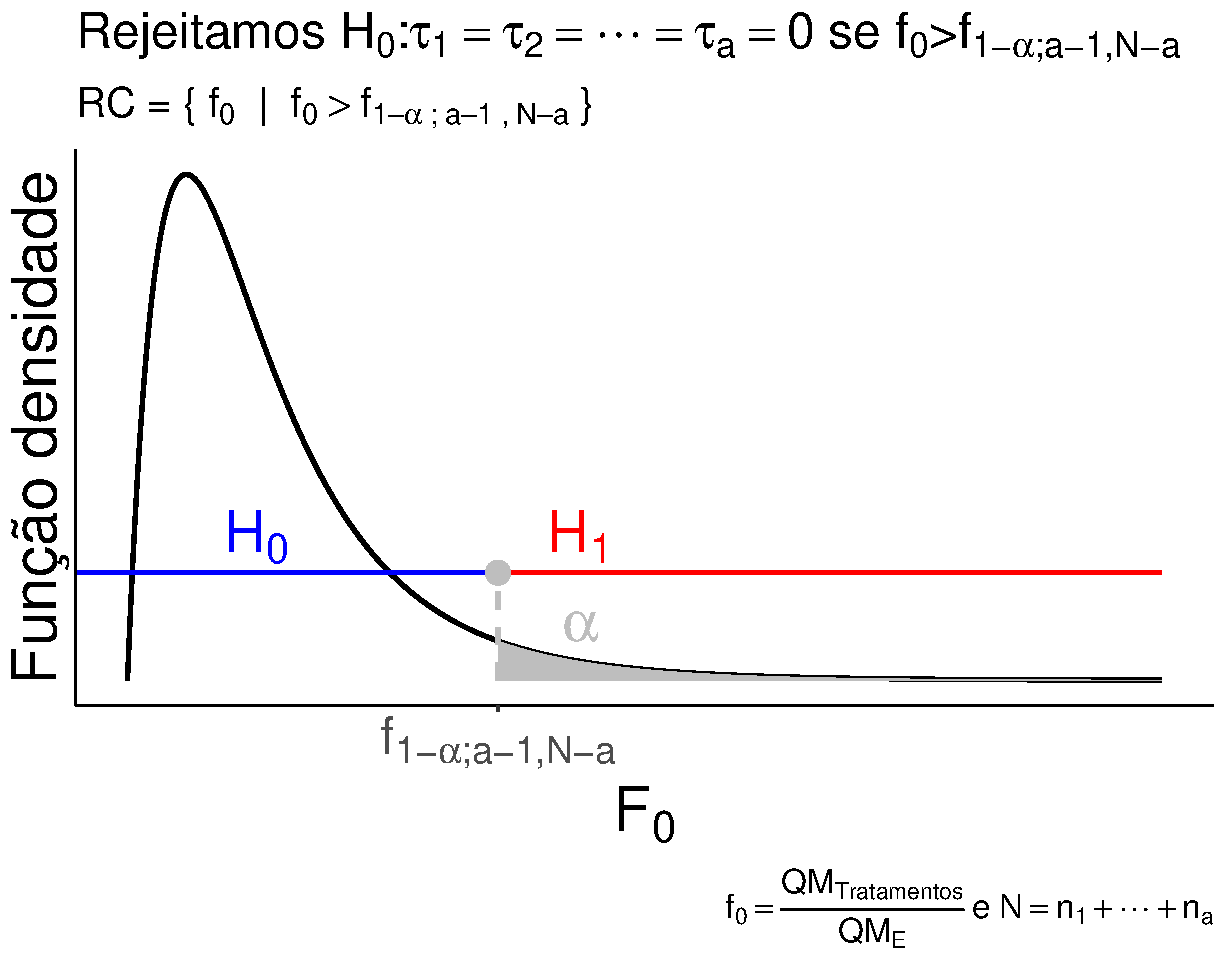
\includegraphics[width=0.70\linewidth]{figure/anova-test-unbalanced.pdf}
	\caption{Região crítica para ANOVA.}
\end{figure}
\end{frame}

\begin{frame}{ANOVA: Checando as suposições do modelo.}

\small
\begin{block}{Análise de resíduo}
	Depois decidir entre $H_0$ e $H_1$, precisamos checar as suposições do modelo:
	\begin{enumerate}[(a)]
		\item $\epsilon_{ij}, j=1, \dots, n_i, i=1, \dots, a$ são independentes;
		\item $\epsilon_{ij}, j=1, \dots, n_i, i=1, \dots, a$ tem distribuição normal;
		\item  $\epsilon_{ij}, j=1, \dots, n_i, i=1, \dots, a$ tem variância constante.
	\end{enumerate} 
	
	$\epsilon_{ij} = y_{ij} - \mu + \tau_i  = y_{ij} - \mu + \tau_i, j=1, \dots, n_i, i=1, \dots, a$ não são observáveis pois não conhecemos as médias populacionais dentro de cada tratamento, mas podemos aproximar estas médias populacionais $\mu_i$ por  $\bar{y}_{i\cdot}, i=1, \dots, a$. Assim, podemos definimos os resíduos por
	\begin{align}\label{eq:residuo}
	e_{ij} = y_{ij} - \bar{y}_{i\cdot}, j=1, \dots, n_i, i=1, \dots, a.
	\end{align}
	
	Usando a equação~\eqref{eq:residuo}, podemos usar gráficos para checar \textcolor{blue}{(a)}, \textcolor{blue}{(b)} e \textcolor{blue}{(c)}:
	\begin{enumerate}[(a)]
		\item \textbf{Independência:} cada par $(i+j, e_{ij}), j=1, \dots, n_i, i=1, \dots, a,$ é representado por um ponto no plano cartesiano. Se não existe padrão ou tendência,então assumimos que $\epsilon_{ij}$ são independentes;
		\item \textbf{Normalidade:} cada par $\left(q_{(i+j)}; \frac{e_{(i+j)} - \bar{e}_{\cdot\cdot}}{s_e}  \right)$$, j=1, \dots, n_i, i=1, \dots, a$ é representado por um ponto no plano cartesiano, em que $\Phi(q_{(i+j)}) = \frac{i+j-0,5}{n}$ e $s_e$ é o desvio padrão dos resíduos -- este gráfico é chamado de gráfico de probabilidade normal. Se os pontos estão próximos ou em cima da reta com ângulo $45$ graus, então $\epsilon_{ij}$ tem distribuição normal;
		\item \textbf{Variância constante:} cada par $\left( \bar{y}_{i\cdot}, e_{ij} \right), j=1, \dots, n_i, i=1, \dots, a,$ é representando por um ponto no plano cartesiano. Se não existe padrão ou tendência, então assumimos que $\epsilon_{ij}$ tem variância constante.
	\end{enumerate}
\end{block}
\normalsize

\end{frame}

\begin{frame}{ANOVA}
\begin{block}{Exemplo}
	Um experimento foi realizado para determinar se quatro temperaturas de queima específicas afetam a densidade de um certo tipo de tijolo. Os dados estão na Tabela~\ref{tab:anova-unbalanced}.
	\begin{table}[htbp]
		\centering
		\begin{tabular}{c|ccccccc}
			\toprule[0.05cm]
			Temperatura & \multicolumn{7}{|c}{Densidade}\\ \midrule[0.025cm]
			40  &  21,8 & 21,9 & 21,7 & 21,6 & 21,7 &  21,5 & 21,8\\
			50  & 21,7 &	21,4 & 21,5 & 21,5 &  &  &  \\
			60  & 21,9 &	21,8 & 21,8 & 21,6 & 21,5 &  & \\
			70  & 21,9 &	21,7 & 21,8 & 21,7 & 21,6 & 21,8 &\\
			\bottomrule[0.05cm]
		\end{tabular}
		\caption{Informações do experimento.}
		\label{tab:anova-unbalanced}
	\end{table}
	\begin{enumerate}[(a)]
		\item As temperaturas de queima específicas afetam a densidade de um certo tipo de tijolo? Use $\alpha=5\%$. 
		\item Calcule o valor-p.
		\item Faça uma análise de resíduo.
	\end{enumerate}
\end{block}
\end{frame}

\begin{frame}{ANOVA}

\small
\begin{block}{Solução}
	\textbf{Passo 1)} Queremos testar as hipóteses: $H_0: \tau_1 = \tau_2 = \tau_3 = \tau_4 = 0$ e $H_1: \tau_1^2 +  \tau_2^2 +  \tau_3^2 + \tau_4^2 > 0$;
	
	\textbf{Passo 2)} Nível de significância $\alpha=5\%$;
	
	\textbf{Passo 3)} Rejeitamos $H_0$ se $F_0 = \frac{QM_{Tratamentos}}{QM_E}$. Ou seja, $RC = \left\{ f_0 \mid f_0 > f_{1-\alpha;a-1, N-a} \right\} $;
	
	\textbf{Passo 4)} Note que $n_1+n_2+n_3+n_4=22$ e $a = 4$. Vamos encontrar o valor crítico:
	\begin{itemize}
		\item $P\left( F_{a-1, N-a} \leq f_{1-\alpha;a-1, N-a} \right) = P\left( F_{3, 18} \leq f_{0,95;3, 18} \right) = 1- \alpha = 0,95$, então $f_{0,95;3, 18} = 3,1599$;
	\end{itemize}

	\textbf{Passo 5)} Usando os dados da Tabela~\ref{tab:anova-unbalanced}, obtemos a Tabela ANOVA (mostrada na Tabela~\ref{tab:anova-unbalanced-test}).
	\begin{table}[ht]
		\centering
		\scalebox{0.87}{
		\begin{tabular}{l|cccc}
			\toprule[0.05cm]
			Fatores de variação & Graus de liberdade & Soma de quadrados & Quadrados médios & $F_0$ \\ 
			\midrule[0.025cm]
			Temperatura $^\circ$C & 3 & $SQ_{Tratamento} = 0,139$ & $QM_{Tratamento}=0,046$ & $\frac{QM_{Tratamentos}}{QM_E} = 2,556$  \\ 
			Erro & $18$ & $SQ_E=0,319$ & $QM_E=0,018$ &  \\  \midrule[0.025cm]
			Total & 21 & $SQ_T = 0,458$ & & \\
			\bottomrule[0.05cm]
		\end{tabular}
		}
		\caption{Tabela Anova} 
		\label{tab:anova-unbalanced-test}
	\end{table}
	Lembre que $SQ_{E} = (n_1-1) s_1^2 + (n_2-1) s_2^2 + (n_3-1) s_3^2 + (n_4-1) s_4^2$, $SQ_T = (N-1)s^2$ e $N = n_1+n_2+n_3+n_4$.

	Como $f_0 = 2, 556 \leq 3,15990 = f_{0,95; 3, 23}$, não rejeitamos $H_0$. Ao nível de significância $\alpha=5\%$, não temos evidência estatística para afirmar que as densidades médias para temperaturas de queima específica são diferentes.
\end{block}
\normalsize

\end{frame}

\begin{frame}{ANOVA}


\begin{block}{Solução (valor-p)}
	O valor-p é calculado através de 
	$$p = P\left(F_0 \mid f_0 \mid H_0\right) = 1 - P\left(F_{a-1, N-a} \leq f_0\right),$$
	em que $N = n_1+\cdots + n_a$.
	
	Usando a Tabela~\ref{tab:anova-unbalanced-test}, temos que $a = 4$, $N = 22$ e $f_0 = 2,556$. Então, temos que
	\begin{align*}
	p &= 1 - P\left(F_{a-1, N-a} \leq f_0\right)\\
	&= 1 - P\left( F_{3, 23} \leq  2,556 \right)\\
	&= 1 - 0,9199\\
	&= 0,0801.
	\end{align*}
	
	Como $p=0,0801 \geq \alpha = 0,05$, não rejeitamos $H_0$. Ou seja, não temos evidência estatística para afirmar que as densidades médias são diferentes para as quatro temperaturas de queima específicas.
\end{block}

\end{frame}

\begin{frame}{ANOVA}

\begin{block}{Solução (Análise de resíduo)}
	Primeiro calculamos os resíduos e a média dentro de cada tratamento, conforme mostrado na Tabela~\ref{tab:anova-unbalanced-residuo}.
	\begin{table}[htbp]
		\centering
		\scalebox{0.75}{
		\begin{tabular}{c|ccccccc|c|c}
			\toprule[0.05cm]
			Temperatura & \multicolumn{7}{|c|}{Resíduo} & $\bar{y}_{i\cdot}$ & $s_i^2$ \\ \midrule[0.025cm]
			40  &  0,0857 & 0,1857 & -0,0143 & -0,1143 & -0,0143 & -0,2143 & 0,0857 & 21,7143 & 0,0181 \\
			50  & 0,175 & -0,125 & -0,025 & -0,025 &  &  & & 21,5250 &  0,0158 \\
			60  & 0,18 & 0,08 & 0,08 & -0,12 & -0,22 &  & &  21,7200 & 0,0270\\
			70  & 0,15 & -0,05 & 0,05 & -0,05 & -0,15 & 0,05 & & 21,7500 & 0,0110 \\
			\bottomrule[0.05cm]
		\end{tabular}
		}
		\caption{Informações do experimento.}
		\label{tab:anova-unbalanced-residuo}
	\end{table}

	\begin{enumerate}[(a)]
		\item Na Figura~\ref{fig:qqnorm-unbalanced}, notamos que os pontos estão próximos da reta e concluímos que $\epsilon_{ij}$ tem distribuição normal;
		\item Na Figura~\ref{fig:independence-unbalanced}, não notamos qualquer padrão ou tendência e concluímos que as variáveis aleatórias $\epsilon_{ij}$ são independentes;
		\item Na Figura~\ref{fig:variance-unbalanced}, não notamos qualquer padrão ou tendência e concluímos que a variância é constante para as variáveis aleatórias $\epsilon_{ij}$.
	\end{enumerate}
\end{block}

\end{frame}

\begin{frame}{ANOVA}
	
	\begin{block}{Análise de resíduo}
		\begin{figure}[htbp]
			\centering
			\subfloat[Gráfico de probabilidade normal.]{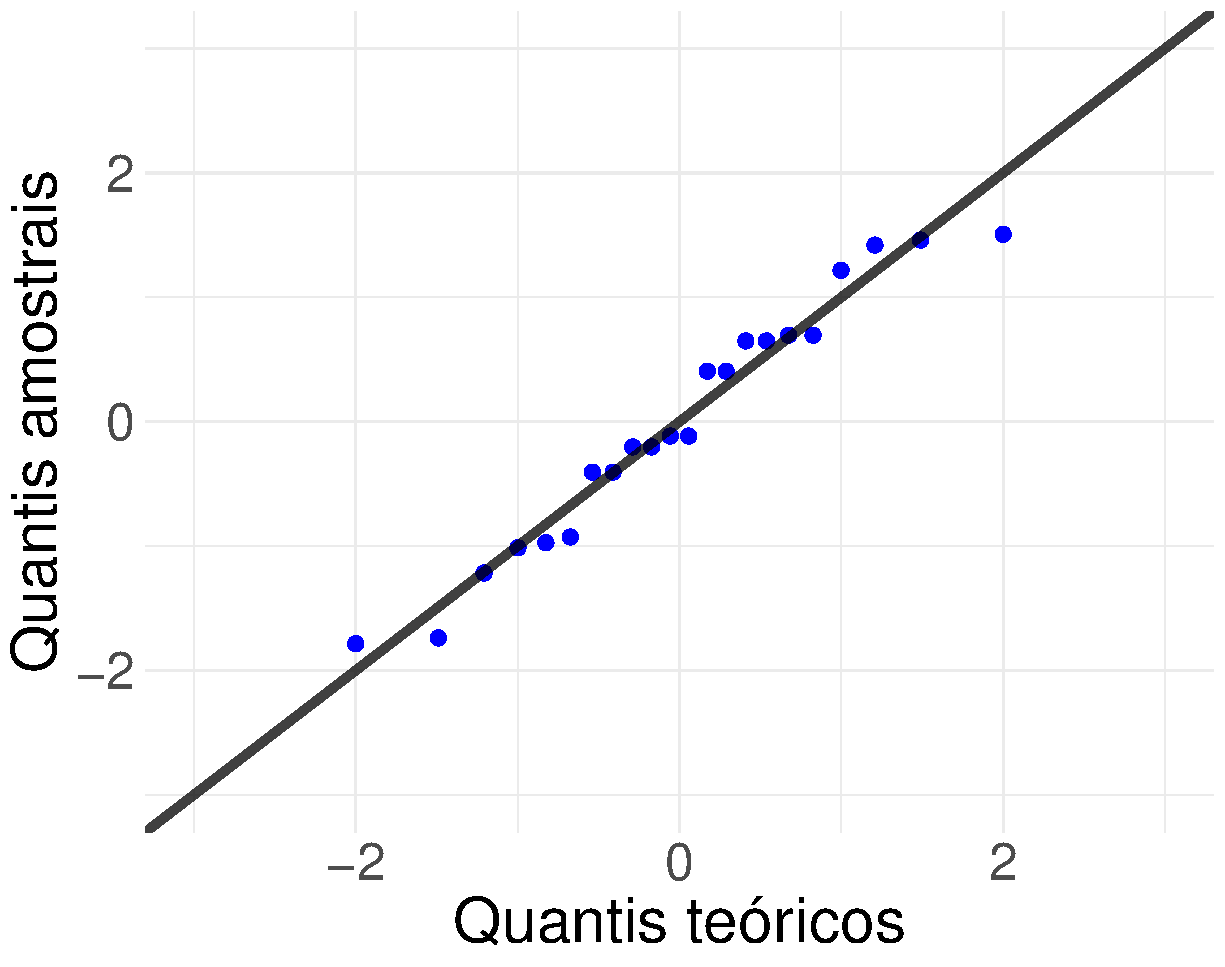
\includegraphics[width=0.33\linewidth]{figure/qqnorm-unbalanced.pdf} \label{fig:qqnorm-unbalanced}}
			\subfloat[Tempo $\times$ Resíduos.]{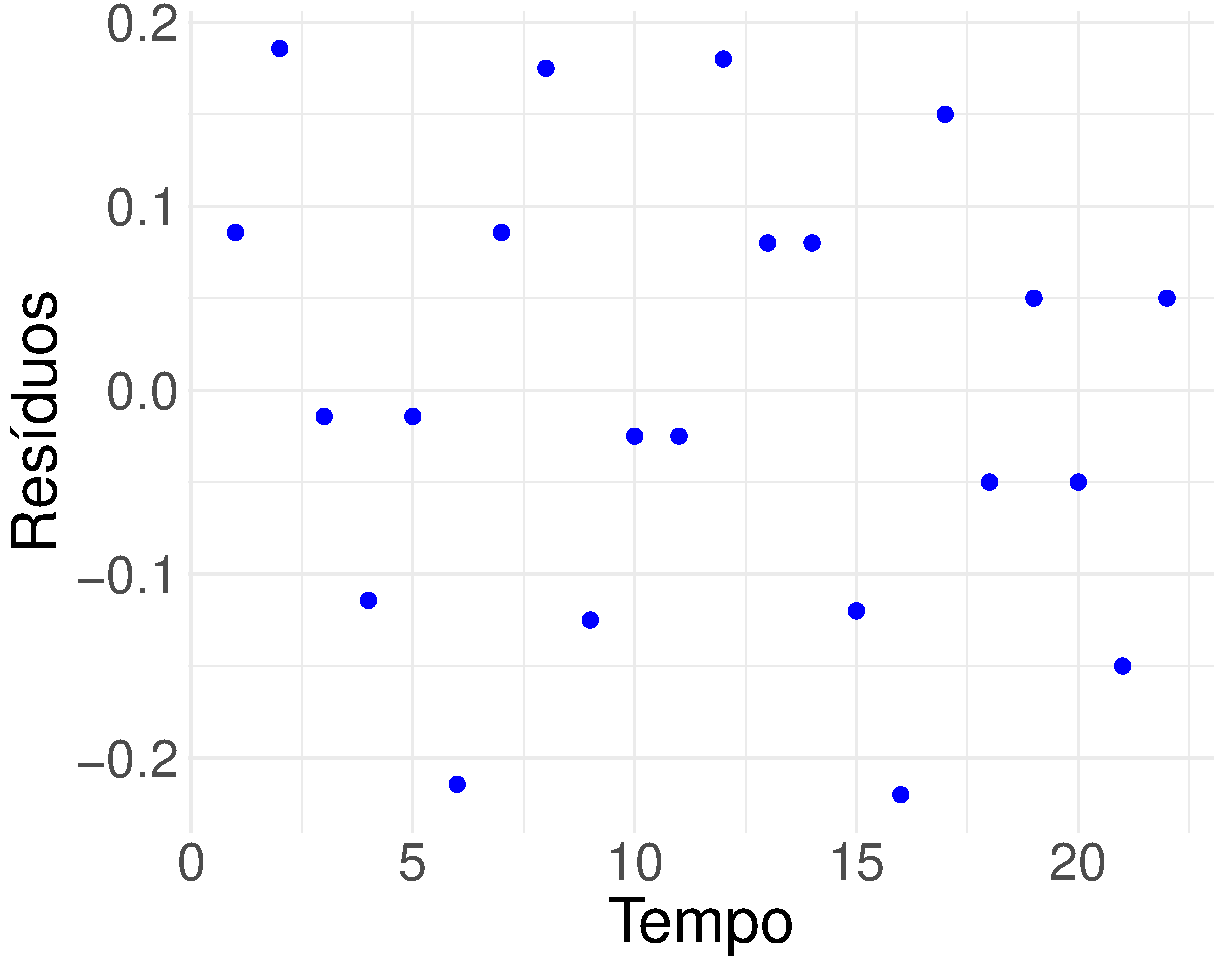
\includegraphics[width=0.33\linewidth]{figure/independence-unbalanced.pdf} \label{fig:independence-unbalanced}}
			\subfloat[$\bar{y}_{i\cdot}$ $\times$ Resíduos.]{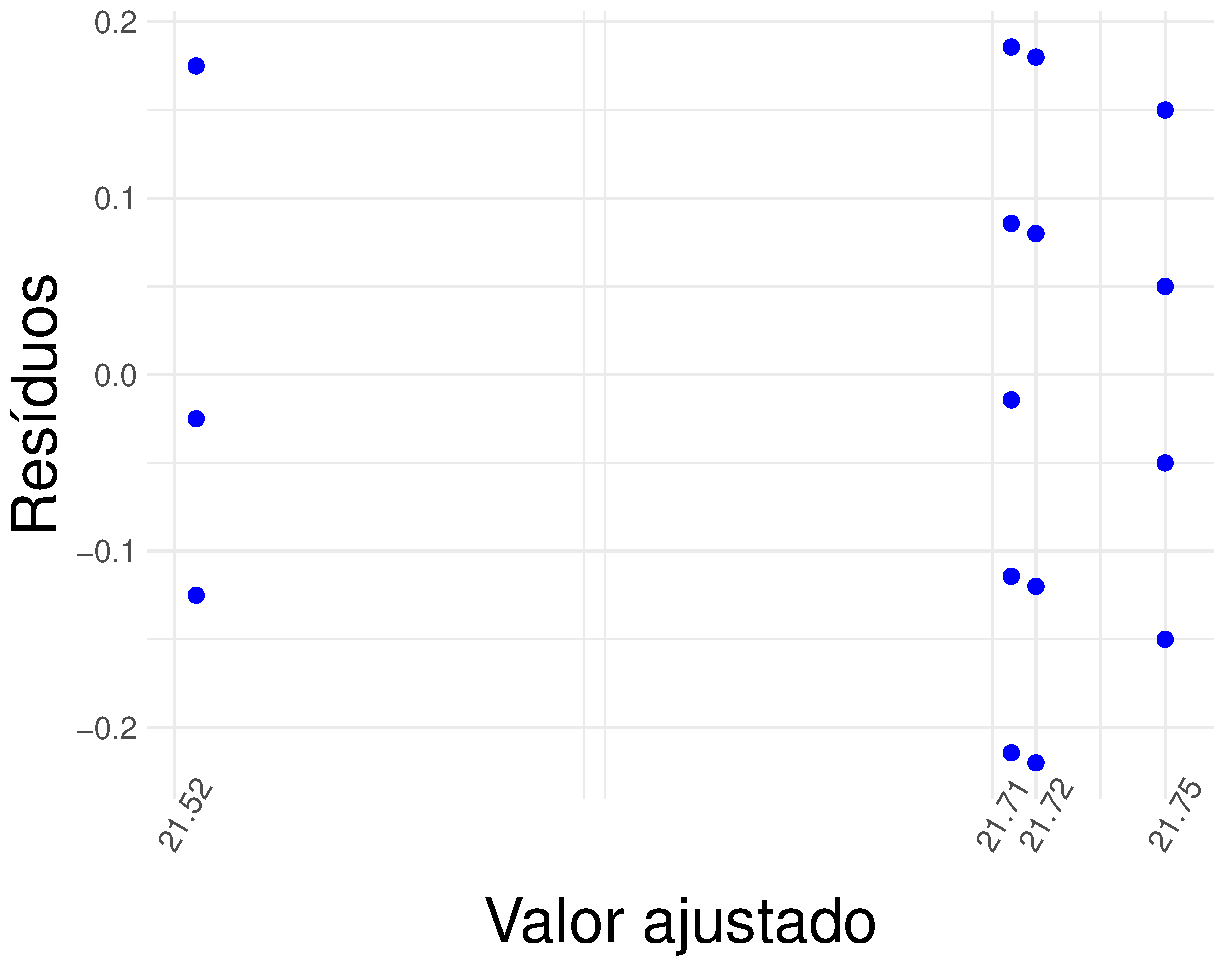
\includegraphics[width=0.33\linewidth]{figure/variance-unbalanced.pdf} \label{fig:variance-unbalanced}}
			\caption{Análise de resíduos.}
		\end{figure}
	\end{block}
	
\end{frame}

\subsection{Poder do teste}

\begin{frame}{Poder do teste (estudos não-balanceados).}


No contexto do modelo da equação~\eqref{eq:anova-unbalanced}, imagine que
\begin{itemize}
	\item Hipóteses: $H_0: \tau_1=\cdots=\tau_a=0$ e $H_1: \tau_1^2 + \cdots + \tau_a^2 > 0$;
	\item $H_1$ é verdade, então $\tau_1^2 + \cdots + \tau_a^2 > 0$;
	\item $F_0 = \frac{QM_{Tratamentos}}{QM_E} \sim F_{a-1, N-a}\left(\Phi^2\right)$, em que $\Phi^2 = \frac{n_1 \tau_1^2 + \cdots + n_a \tau_a^2}{a \sigma^2}$, em que $n_i$ é o número de observações do  Tratamento $i$, $i=1, \dots, a$;
	\item Ao nível de significância $\alpha$, temos $RC = \{ f_0 \mid f_0 > f_{1-\alpha;a-1, N-a}  \}$.
\end{itemize}

Poder do teste é dado por
\begin{align*}
\textcolor{important}{1-\beta}  = 1 - P\left( F_0 \leq f_{1-\alpha;a-1, N-a} \mid H_0 \right) = 1- P\left( F_{a-1, N-a}\left( \Phi^2 \right) \leq f_{1-\alpha;a-1, N-a}  \right)
\end{align*}
em que $N = n_1 + \cdots + n_a$. A \textcolor{important}{Função Poder}, dado o tamanho da amostra $N$, o número de tratamentos $a$ e os tamanhos dos tratamentos são $n$, é  $\pi: (0, \infty) \longrightarrow [0,1]$ dada por
\begin{align*}
\pi(\Phi^2) = 1- P\left( F_{a-1, N-a}\left( \Phi^2\right) \leq f_{1-\alpha;a-1, N-a}  \right), \qquad \Phi^2 \in (0,\infty).
\end{align*}
Alguns livros chamada a Função Poder de \textcolor{important}{Curva de Característica Operacional.}
\end{frame}

\begin{frame}{Poder do teste (estudos não-balanceados).}

\begin{block}{Exemplo}
	Um experimento foi realizado para determinar se quatro temperaturas de queima específicas afetam a densidade de um certo tipo de tijolo. Algumas informações estão na Tabela~\ref{tab:anova-unbalanced-power}. Qual o poder do teste? Use $\alpha=5\%$.
	\begin{table}[htbp]
		\centering
		\begin{tabular}{c|ccc}
			\toprule[0.05cm]
			Temperatura & $n_i$ & $\mu_i$ & $\sigma_i$ \\ \midrule[0.025cm]
			40  & 4 & 21 & 2 \\
			50  & 5 & 14 & 2  \\
			60  & 6 & 15 & 2 \\
			70  & 4 & 25 & 2\\ \midrule[0.025cm]
			    &   & $\mu = 21$ & $\sigma^2 = 2$\\
			\bottomrule[0.05cm]
		\end{tabular}
		\caption{Informações do experimento.}
		\label{tab:anova-unbalanced-power}
	\end{table}
	Note que $\mu_i = \mu + \tau_i$ é a média de cada tratamento, $\sigma^2_i$ é a variância de cada  tratamento, $\mu$ é a média total e $\sigma^2$ é a variância total.
\end{block}

\end{frame}

\begin{frame}{Poder do teste (estudos não-balanceados).}
	\begin{block}{Solução}
		Primeiro vamos calcular os efeitos dentro de cada tratamento:
		\begin{align*}
			\tau_1 &= \mu_i - \mu = 21 - 21 = 0 \qquad & \tau_2 = \mu_2 - \mu = 14 - 21 = -7\\
			\tau_3 &= \mu_i - \mu = 15 - 21 = -6 \qquad & \tau_4= \mu_4 - \mu = 25 - 21 = 4
		\end{align*}
		Então, o parâmetro de não-centralidade é dada por
		\begin{align*}
		\Phi^2 = \frac{n_1\tau_1^2 + \cdots + n_a\tau_a^2}{a \sigma^2} = \frac{4\cdot 0^2 + 5 \cdot (-7)^2 + 6 \cdot (-6)^2 + 4 \cdot 4^2}{4 \cdot 2} = 65,625.
		\end{align*}
		
		Vamos encontrar o quantil da distribuição $F$:
		\begin{itemize}
			\item $P(F_{a-1, N-a} \leq f_{1-\alpha;a-1, N-a}) = P(F_{3, 15} \leq f_{0,95;3, 15}) = 1 - \alpha = 0,95$, então $f_{0,95;3, 15}=3,2874$.
		\end{itemize}
	
	Então o poder do teste é dado por
	\begin{align*}
		1- \beta &= 1 - P(F_{a-1, N - a}(\Phi^2) \leq f_{1-\alpha;a-1, N-a}) = 1 - P\left( F_{3, 15}(65,625) \leq 3,2874 \right)\\
		&= 1.
	\end{align*}
	\end{block}
\end{frame}

\subsection{Intervalo de confiança para médias}

\begin{frame}{Intervalo de confiança para médias}

Considere o modelo dado por
$$Y_{ij} = \mu + \tau_i  + \epsilon_{ij}, \qquad \epsilon_{ij} \sim N(0, \sigma^2), \qquad j=1, \dots, n_i, i=1, \dots, a.$$
Neste contexto, a média para cada tratamento é $\mu_i$ e pode ser aproximada por $\bar{y}_{i\cdot} = \frac{y_{i1} + y_{i2} + \cdots + y_{in_i}}{n_i} $. Pode-se provar que
\begin{align*}
T = \frac{\bar{Y}_{i\cdot} - \mu_i}{\sqrt{\frac{QM_E}{n_i}}} \sim t_{N - a}.
\end{align*}
em que $\mu_i=\mu+\tau_i,i =1, \dots, a$ e $N = n_1 + \cdots + n_a$. Lembre que $\espe\left[QM_E\right] = \sigma^2$. Dado o coeficiente de confiança $\gamma=1-alpha$, temos que
\begin{align*}
\gamma = P\left( t_{\frac{\alpha}{2};N - a} \leq \frac{\bar{Y}_{i\cdot} - \mu_i}{\sqrt{\frac{QM_E}{n_i}}} \leq t_{1-\frac{\alpha}{2};N - a}  \right),
\end{align*}
e o intervalo de confiança para a média $\mu_i$ do tratamento  $i$ é dado
\begin{align*}
IC(\mu_i, \gamma) = \left( t_{\frac{\alpha}{2};N - a} \sqrt{\frac{QM_E}{n_i}} + \bar{y}_{i\cdot}; t_{1-\frac{\alpha}{2};N - a} \sqrt{\frac{QM_E}{n_i}} + \bar{y}_{i\cdot} \right).
\end{align*}
\end{frame}

\begin{frame}{Intervalo de confiança para as médias.}
\begin{block}{Exemplo}
	Um experimento foi realizado para determinar se quatro temperaturas de queima específicas afetam a densidade de um certo tipo de tijolo. Os dados estão na Tabela~\ref{tab:anova-unbalanced-ic-medias}. Construa um intervalo de confiança para a densidade média do tijolo para temperatura de queima igual a $40$. Use $\gamma = 99\%$.
	\begin{table}[htbp]
		\centering
		\scalebox{0.8}{
		\begin{tabular}{c|ccccccc|c|c}
			\toprule[0.05cm]
			Temperatura & \multicolumn{7}{|c|}{Densidade} & $\bar{y}_{i\cdot}$ & $s_i^2$\\ \midrule[0.025cm]
			40  &  21,8 & 21,9 & 21,7 & 21,6 & 21,7 &  21,5 & 21,8 & 21,7143 & 0,0181 \\
			50  & 21,7 &	21,4 & 21,5 & 21,5 &  &  & & 21,5250 & 0,0158 \\
			60  & 21,9 &	21,8 & 21,8 & 21,6 & 21,5 &  & & 21,7200 & 0,0270 \\
			70  & 21,9 &	21,7 & 21,8 & 21,7 & 21,6 & 21,8 & & 21,7500 & 0,0110 \\ \midrule[0.025cm]
			\multicolumn{8}{c|}{  } & $\bar{y}_{\cdot\cdot}=21,6909$ & $s^2=0,0218$ \\
			\bottomrule[0.05cm]
		\end{tabular}
		}
		\caption{Informações do experimento.}
		\label{tab:anova-unbalanced-ic-medias}
	\end{table}
\end{block}
\end{frame}

\begin{frame}{Intervalo de confiança para as médias.}

\scriptsize
\begin{block}{Solução}
	Primeiro vamos calcular a tabela anova. Mostramos o resultado na Tabela~\ref{tab:anova-table-unbalanced}.
	\begin{table}[ht]
		\centering
		\scalebox{0.87}{
		\begin{tabular}{l|cccc}
			\toprule[0.05cm]
			Fatores de variação & Graus de liberdade & Soma de quadrados & Quadrados médios & $F_0$ \\ 
			\midrule[0.025cm]
			Temperatura $^\circ$C & 3 & $SQ_{Tratamento} = 0,139$ & $QM_{Tratamento}=0,046$ & $\frac{QM_{Tratamentos}}{QM_E} = 2,556$  \\ 
			Erro & $18$ & $SQ_E=0,319$ & $QM_E=0,018$ &  \\  \midrule[0.025cm]
			Total & 21 & $SQ_T = 0,458$ & & \\
			\bottomrule[0.05cm]
		\end{tabular}
		}
		\caption{Tabela ANOVA.} 
		\label{tab:anova-table-unbalanced}
	\end{table}
	
	Note que $\gamma = 0,99 = 1 - \alpha$, $\alpha = 0,05$, $a=4$, $N-a=18$ e $N = 22$. Vamos calcular os quantis da distribuição $t$-Student:
	\begin{itemize}
		\item $P\left( t_{N - a} \leq t_{\frac{\alpha}{2}, N - a} \right) = P\left( t_{18} \leq t_{0,005; 18} \right) = \frac{\alpha}{2} = 0,025$, então $t_{0,005; 18} = -2,878$;
		\item $P\left( t_{N - a} \leq t_{\frac{\alpha}{2}, N - a} \right) = P\left( t_{18} \leq t_{0,995; 18} \right) = 1- \frac{\alpha}{2} = 0,995$, então $t_{0,995; 20} =   2,878$.
	\end{itemize}
	
	Então o intervalo de confiança é dado por
	\begin{align*}
	IC(\mu_1, \gamma) &= \left( \bar{y}_{1\cdot} + t_{\frac{\alpha}{2};N - a} \sqrt{\frac{QM_E}{n_1}};  \bar{y}_{1\cdot} + t_{1-\frac{\alpha}{2};N - a} \sqrt{\frac{QM_E}{n_1}}  \right)= \left( 21,7143 - 2,878 \sqrt{\frac{0,018}{7}}; 21,7143 + 2,878 \sqrt{\frac{0,018}{7}} \right)\\ 
	&= \left( 21,57; 21,86 \right).
	\end{align*}
	Então, a densidade média população dos tijolos com temperatura de queima igual a $40$ está entre $21,57$ e $21,86$.	
\end{block}
\normalsize

\end{frame}

\subsection{Intervalo de confiança para diferenças das médias}

\begin{frame}{Intervalo de confiança para diferenças das médias}

Considere o modelo dado por
$$Y_{ij} = \mu + \tau_i  + \epsilon_{ij}, \qquad \epsilon_{ij} \sim N(0, \sigma^2), \qquad j=1, \dots, n_i, i=1, \dots, a.$$
Neste contexto, a média para cada tratamento é $\mu_i$ e pode ser aproximada por $\bar{y}_{i\cdot} = \frac{y_{i1} + y_{i2} + \cdots + y_{in_i}}{n_i}$. Pode-se provar que
\begin{align*}
T = \frac{(\bar{Y}_{i\cdot} - \bar{Y}_{j\cdot}) - (\mu_i - \mu_j)}{\sqrt{QM_E\left(\frac{1}{n_i} + \frac{1}{n_j} \right)}} \sim t_{N - a}.
\end{align*}
em que $\mu_i=\mu+\tau_i,i =1, \dots, a$ e $N = n_1 + \cdots + n_a$. Lembre que $\espe\left[QM_E\right] = \sigma^2$. Dado o coeficiente de confiança $\gamma=1-\alpha$, temos que
\begin{align*}
\gamma = P\left( t_{\frac{\alpha}{2};N - a} \leq \frac{(\bar{Y}_{i\cdot} - \bar{Y}_{j\cdot}) - (\mu_i - \mu_j)}{\sqrt{QM_E\left(\frac{1}{n_i} + \frac{1}{n_j} \right)}} \leq t_{1-\frac{\alpha}{2};N - a}  \right),
\end{align*}
e o intervalo de confiança para a média $\mu_i$ do tratamento  $i$ é dado
\footnotesize
\begin{align*}
IC(\mu_i - \mu_j, \gamma) = \left( t_{\frac{\alpha}{2};N - a} \sqrt{QM_E\left(\frac{1}{n_i} + \frac{1}{n_j} \right)} + (\bar{y}_{i\cdot} - \bar{y}_{j\cdot}); t_{1-\frac{\alpha}{2};N - a} \sqrt{QM_E\left(\frac{1}{n_i} + \frac{1}{n_j} \right)} + (\bar{y}_{i\cdot} - \bar{y}_{j\cdot}) \right).
\end{align*}
\normalsize

\end{frame}

\begin{frame}{Intervalo de confiança para diferenças das médias}

\begin{block}{Exemplo}
	Um experimento foi realizado para determinar se quatro temperaturas de queima específicas afetam a densidade de um certo tipo de tijolo. Os dados estão na Tabela~\ref{tab:anova-unbalanced-ic-dif-medias}. Construa um intervalo de confiança para a diferença das densidades médias do tijolo para temperaturas de queima igual a $40$ e $60$. Use $\gamma = 99\%$.
	\begin{table}[htbp]
		\centering
		\scalebox{0.8}{
			\begin{tabular}{c|ccccccc|c|c}
				\toprule[0.05cm]
				Temperatura & \multicolumn{7}{|c|}{Densidade} & $\bar{y}_{i\cdot}$ & $s_i^2$\\ \midrule[0.025cm]
				40  &  21,8 & 21,9 & 21,7 & 21,6 & 21,7 &  21,5 & 21,8 & 21,7143 & 0,0181 \\
				50  & 21,7 &	21,4 & 21,5 & 21,5 &  &  & & 21,5250 & 0,0158 \\
				60  & 21,9 &	21,8 & 21,8 & 21,6 & 21,5 &  & & 21,7200 & 0,0270 \\
				70  & 21,9 &	21,7 & 21,8 & 21,7 & 21,6 & 21,8 & & 21,7500 & 0,0110 \\ \midrule[0.025cm]
				\multicolumn{8}{c|}{  } & $\bar{y}_{\cdot\cdot}=21,6909$ & $s^2=0,0218$ \\
				\bottomrule[0.05cm]
			\end{tabular}
		}
		\caption{Informações do experimento.}
		\label{tab:anova-unbalanced-ic-dif-medias}
	\end{table}
\end{block}

\end{frame}

\begin{frame}{Intervalo de confiança para diferenças das médias}

\scriptsize
\begin{block}{Solução}
	Primeiro vamos calcular a tabela anova. Mostramos o resultado na Tabela~\ref{tab:anova-table-unbalanced-dif}.
	\begin{table}[ht]
		\centering
		\scalebox{0.87}{
			\begin{tabular}{l|cccc}
				\toprule[0.05cm]
				Fatores de variação & Graus de liberdade & Soma de quadrados & Quadrados médios & $F_0$ \\ 
				\midrule[0.025cm]
				Temperatura $^\circ$C & 3 & $SQ_{Tratamento} = 0,139$ & $QM_{Tratamento}=0,046$ & $\frac{QM_{Tratamentos}}{QM_E} = 2,556$  \\ 
				Erro & $18$ & $SQ_E=0,319$ & $QM_E=0,018$ &  \\  \midrule[0.025cm]
				Total & 21 & $SQ_T = 0,458$ & & \\
				\bottomrule[0.05cm]
			\end{tabular}
		}
		\caption{Tabela ANOVA.} 
		\label{tab:anova-table-unbalanced-dif}
	\end{table}
	
	Note que $\gamma = 0,99 = 1 - \alpha$, $\alpha = 0,05$, $a=4$, $N-a=18$ e $N = 22$. Vamos calcular os quantis da distribuição $t$-Student:
	\begin{itemize}
		\item $P\left( t_{N - a} \leq t_{\frac{\alpha}{2}, N - a} \right) = P\left( t_{18} \leq t_{0,005; 18} \right) = \frac{\alpha}{2} = 0,025$, então $t_{0,005; 18} = -2,878$;
		\item $P\left( t_{N - a} \leq t_{\frac{\alpha}{2}, N - a} \right) = P\left( t_{18} \leq t_{0,995; 18} \right) = 1- \frac{\alpha}{2} = 0,995$, então $t_{0,995; 20} =   2,878$.
	\end{itemize}
	
	Então o intervalo de confiança é dado por:
	\begin{align*}
	IC(\mu_1-\mu_3, \gamma) &= \left( \left(\bar{y}_{1\cdot} - \bar{y}_{3\cdot}\right) + t_{\frac{\alpha}{2};N - a} \sqrt{QM_E\left(\frac{1}{n_1} + \frac{1}{n_2}\right)};  \left(\bar{y}_{1\cdot} - \bar{y}_{3\cdot}\right) + t_{1-\frac{\alpha}{2};N - a} \sqrt{QM_E\left(\frac{1}{n_1} + \frac{1}{n_2}\right)}  \right)\\
	&= \left( \left(21,7143 - 21,72\right) - 2,878 \sqrt{0,018\left(\frac{1}{7} + \frac{1}{5}\right)}; \left(21,7143 - 21,72\right) + 2,878 \sqrt{0,018\left(\frac{1}{7} + \frac{1}{5}\right)} \right) = \left( -0,23; 0,22 \right).
	\end{align*}
	Então, como $0 \in IC(\mu_1-\mu_3, 99\%)$, as densidades médias dos tijolos para temperaturas de queima iguais a $40$ e $60$ são iguais.	
\end{block}
\normalsize

\end{frame}

\end{document}
